Os resultados apresentam aspectos relacionados ao sistema lógico, seu design e detalhes técnicos que impactam diretamente na implantação do sistema. Para isto, foram realizadas a prototipação de interfaces, diagrama do banco de dados, diagrama do sistema, análise do projeto no Canvas e desenvolvimento de uma plataforma web no Apex.

\subsection*{PROTOTIPAÇÃO DE INTERFACES}

A prototipação do software foi realizada no Figma. Com o objetivo de desenvolver um sistema simples e intuitivo, foram criadas telas o mais amigáveis possíveis (para que o sistema um público abrangente com diferentes tipos de escolaridade). A fonte utilizada foi a Code Tommy, uma fonte gratuita, sem serifa muito parecida com fontes tradicionais do mercado. O esquema de cores foi baseado em tons de verde que, além de estarem relacionados com o tema do trabalho, também visam o conforto visual do usuário. É um conceito visual adotado em toda etapa de prototipação de interfaces.

\begin{figure}[!h]
\centering
\caption{Splash screen}%
\label{fig:picture1}
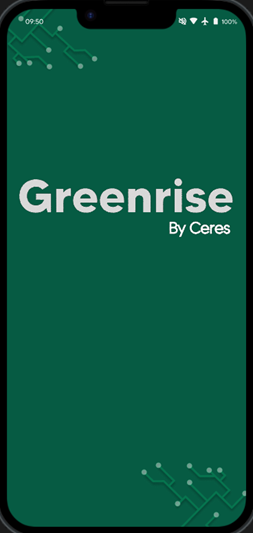
\includegraphics[scale=1]{Illustrations/Picture1.png}
\SourceOrNote{Autoria Própria (2024)}
\end{figure}

Foi criada uma Splash screen (tela de abertura) sem botões e apenas uma animação do logotipo do projeto e um leve delay para a tela seguinte.

\begin{figure}[!h]
\centering
\caption{Tela de login}
\label{fig:picture2}
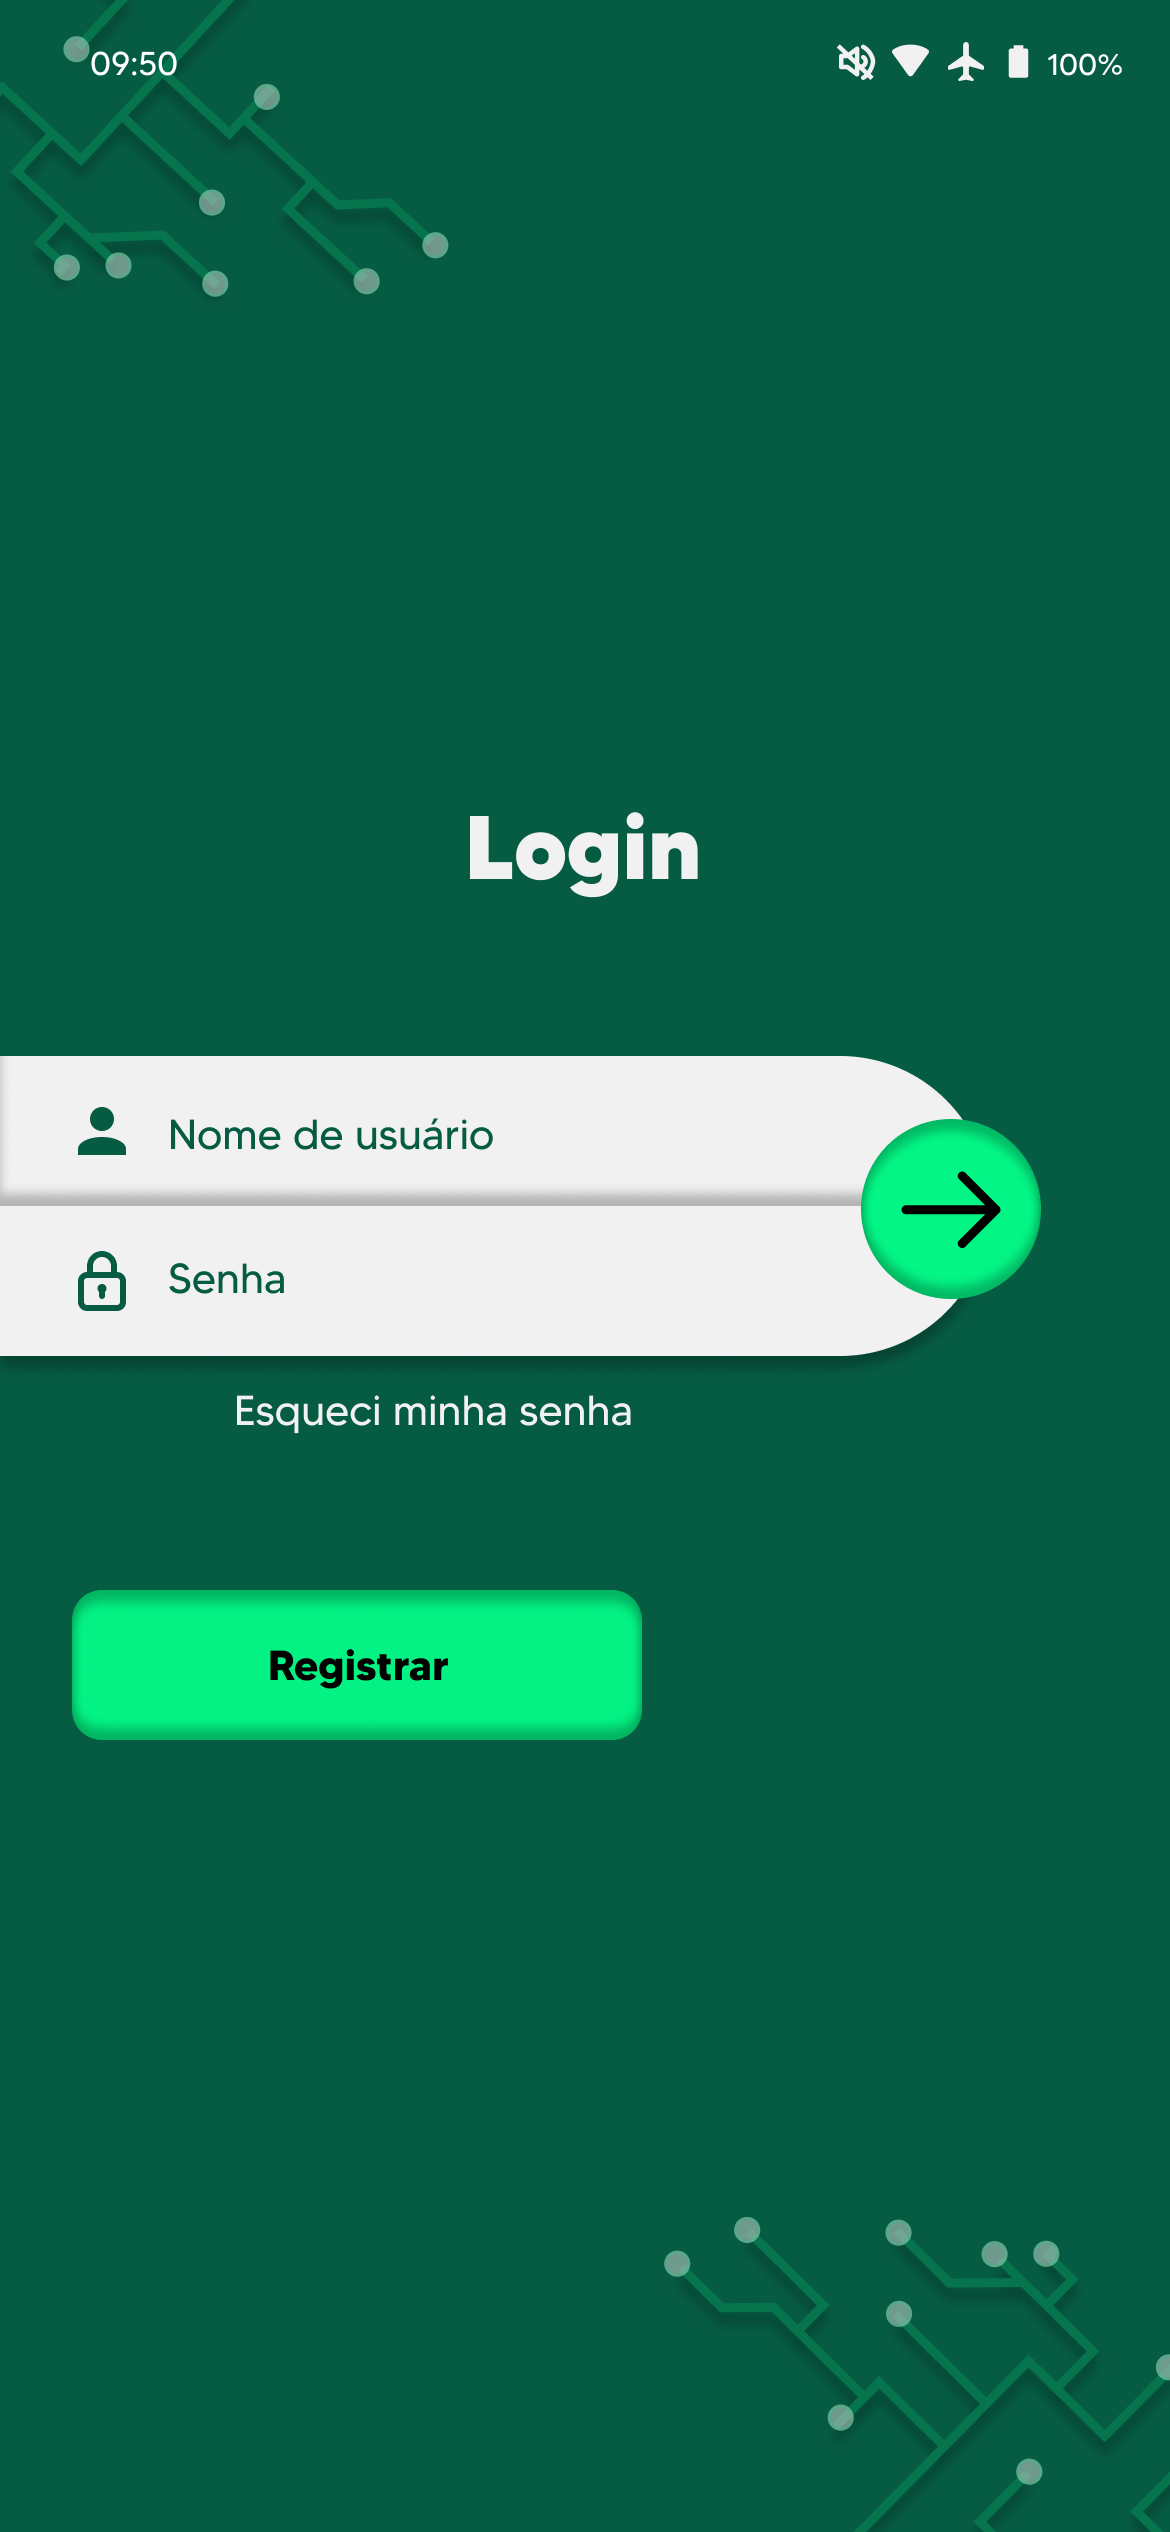
\includegraphics[scale=0.3]{Illustrations/Picture2.png}
\SourceOrNote{Autoria Própria (2024)}
\end{figure}
  
Após a tela de abertura temos a tela de login, onde o usuário deve inserir o usuário cadastrado e a senha nos campos designados. Caso tenha esquecido a senha, o sistema oferece ao usuário a opção de recuperação da mesma. Se o usuário não estiver cadastrado, ele deve clicar em “Registrar”, onde será encaminhado para a tela de registro.

\begin{figure}[!h]
\centering
\caption{Tela de registro}
\label{fig:picture3}
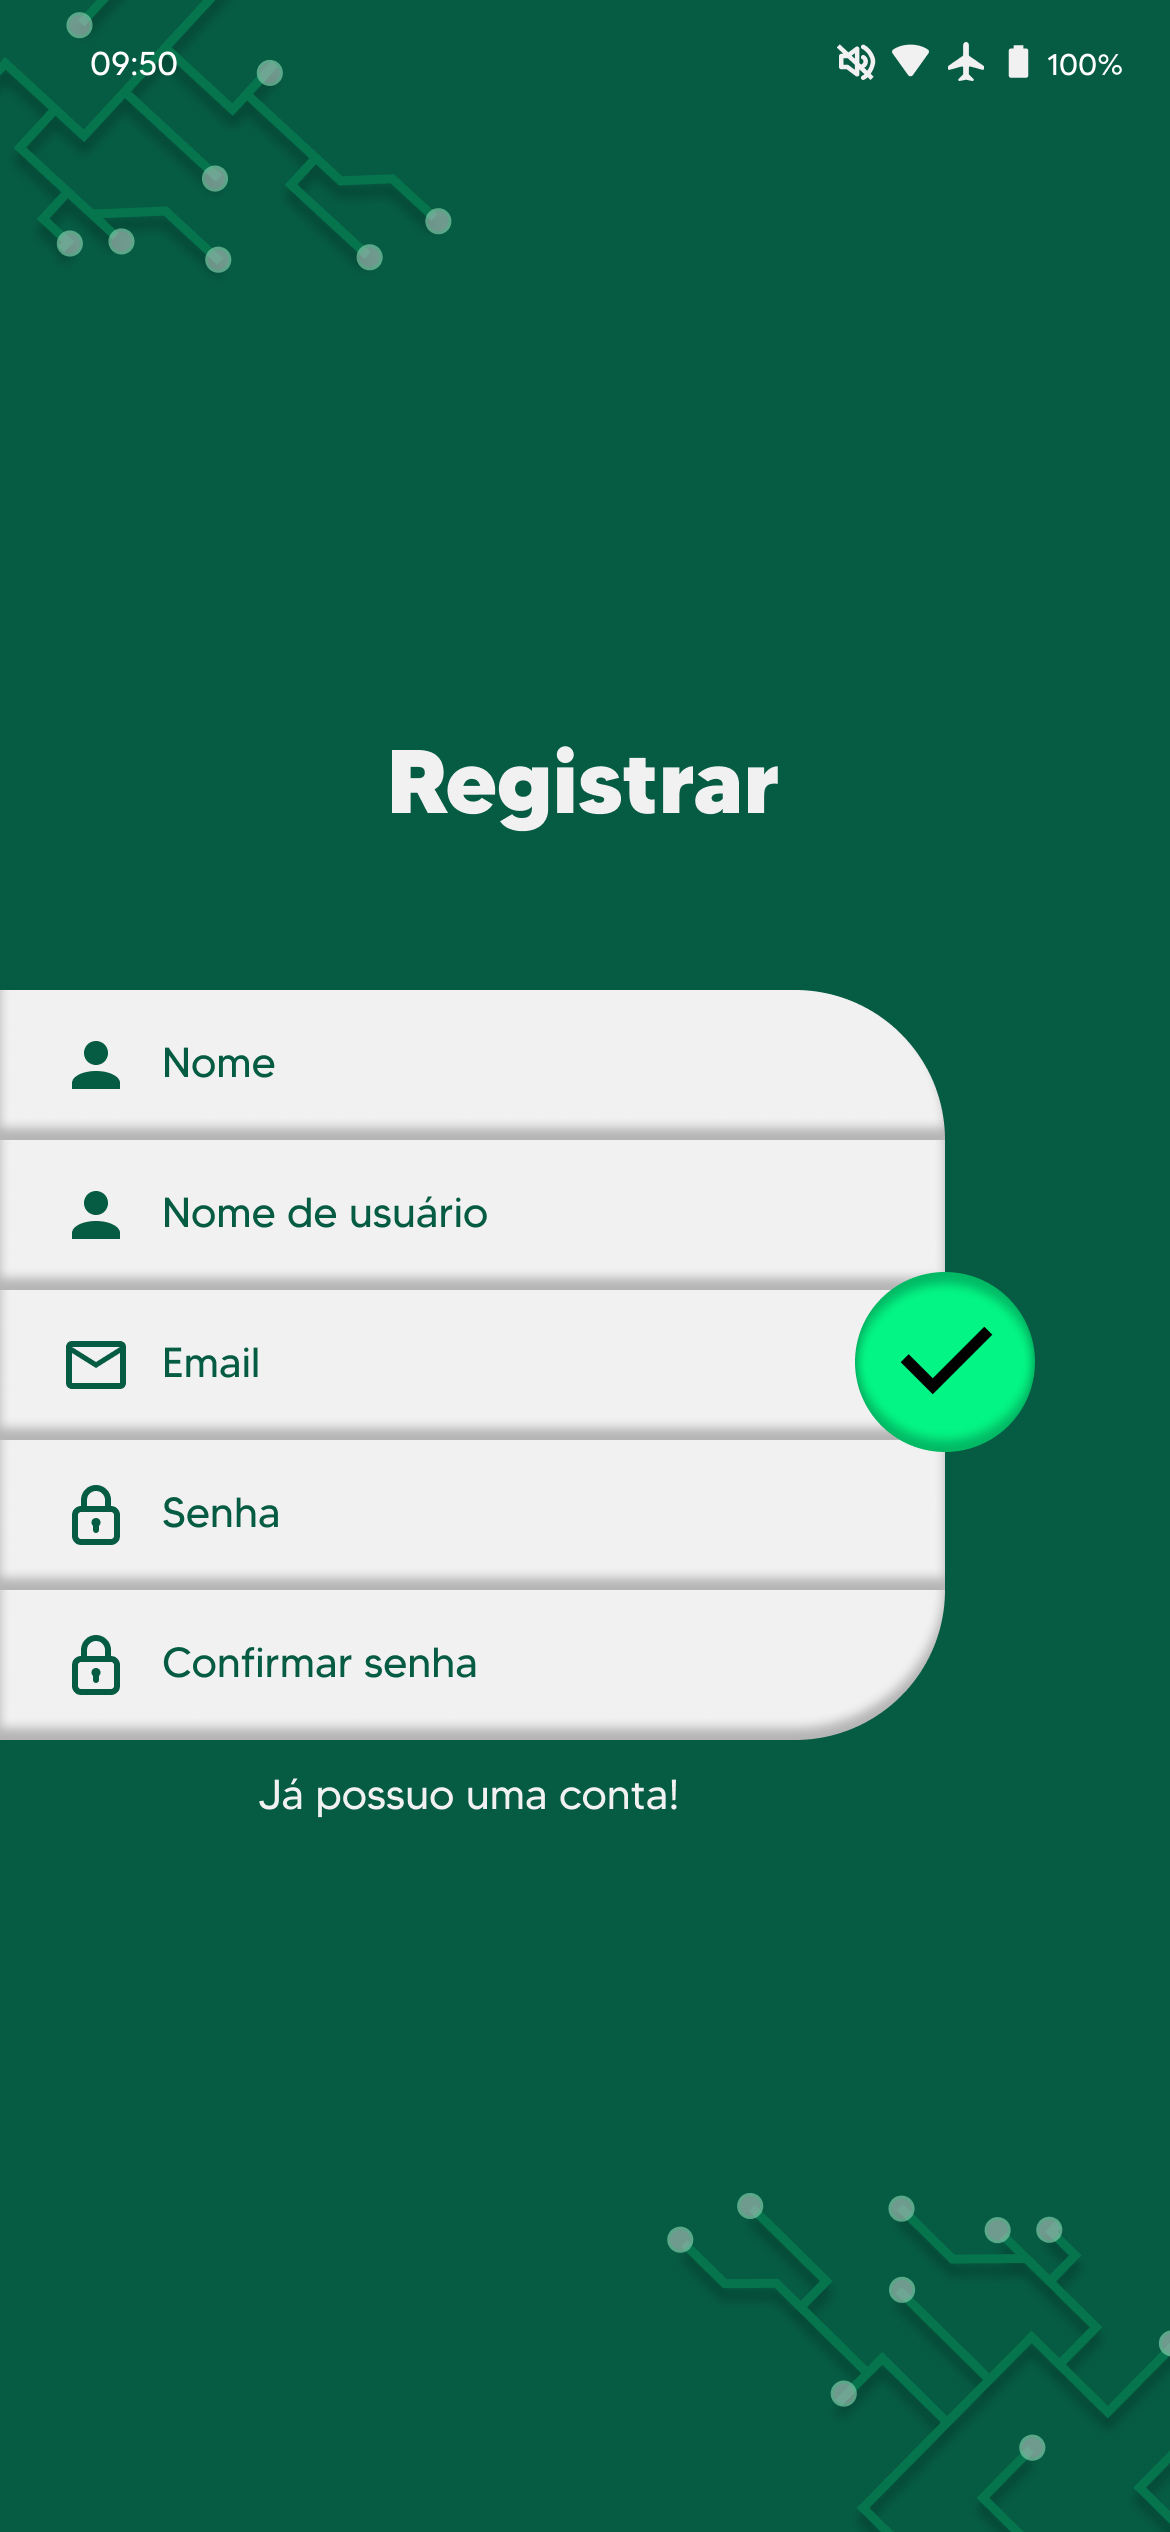
\includegraphics[scale=0.3]{Illustrations/Picture3.png}
\SourceOrNote{Autoria Própria (2024)}
\end{figure}

Caso o usuário precise se cadastrar ele será encaminhado para tela de registro. Para se registrar basta preencher os campos com seu nome completo, um nome de usuário, email, criar uma senha e confirmar a senha criada. Logo após, basta criar no ícone de confirmação para entrar no aplicativo.

\begin{figure}[!h]
\centering
\caption{Tela de boas-vindas}
\label{fig:picture4}
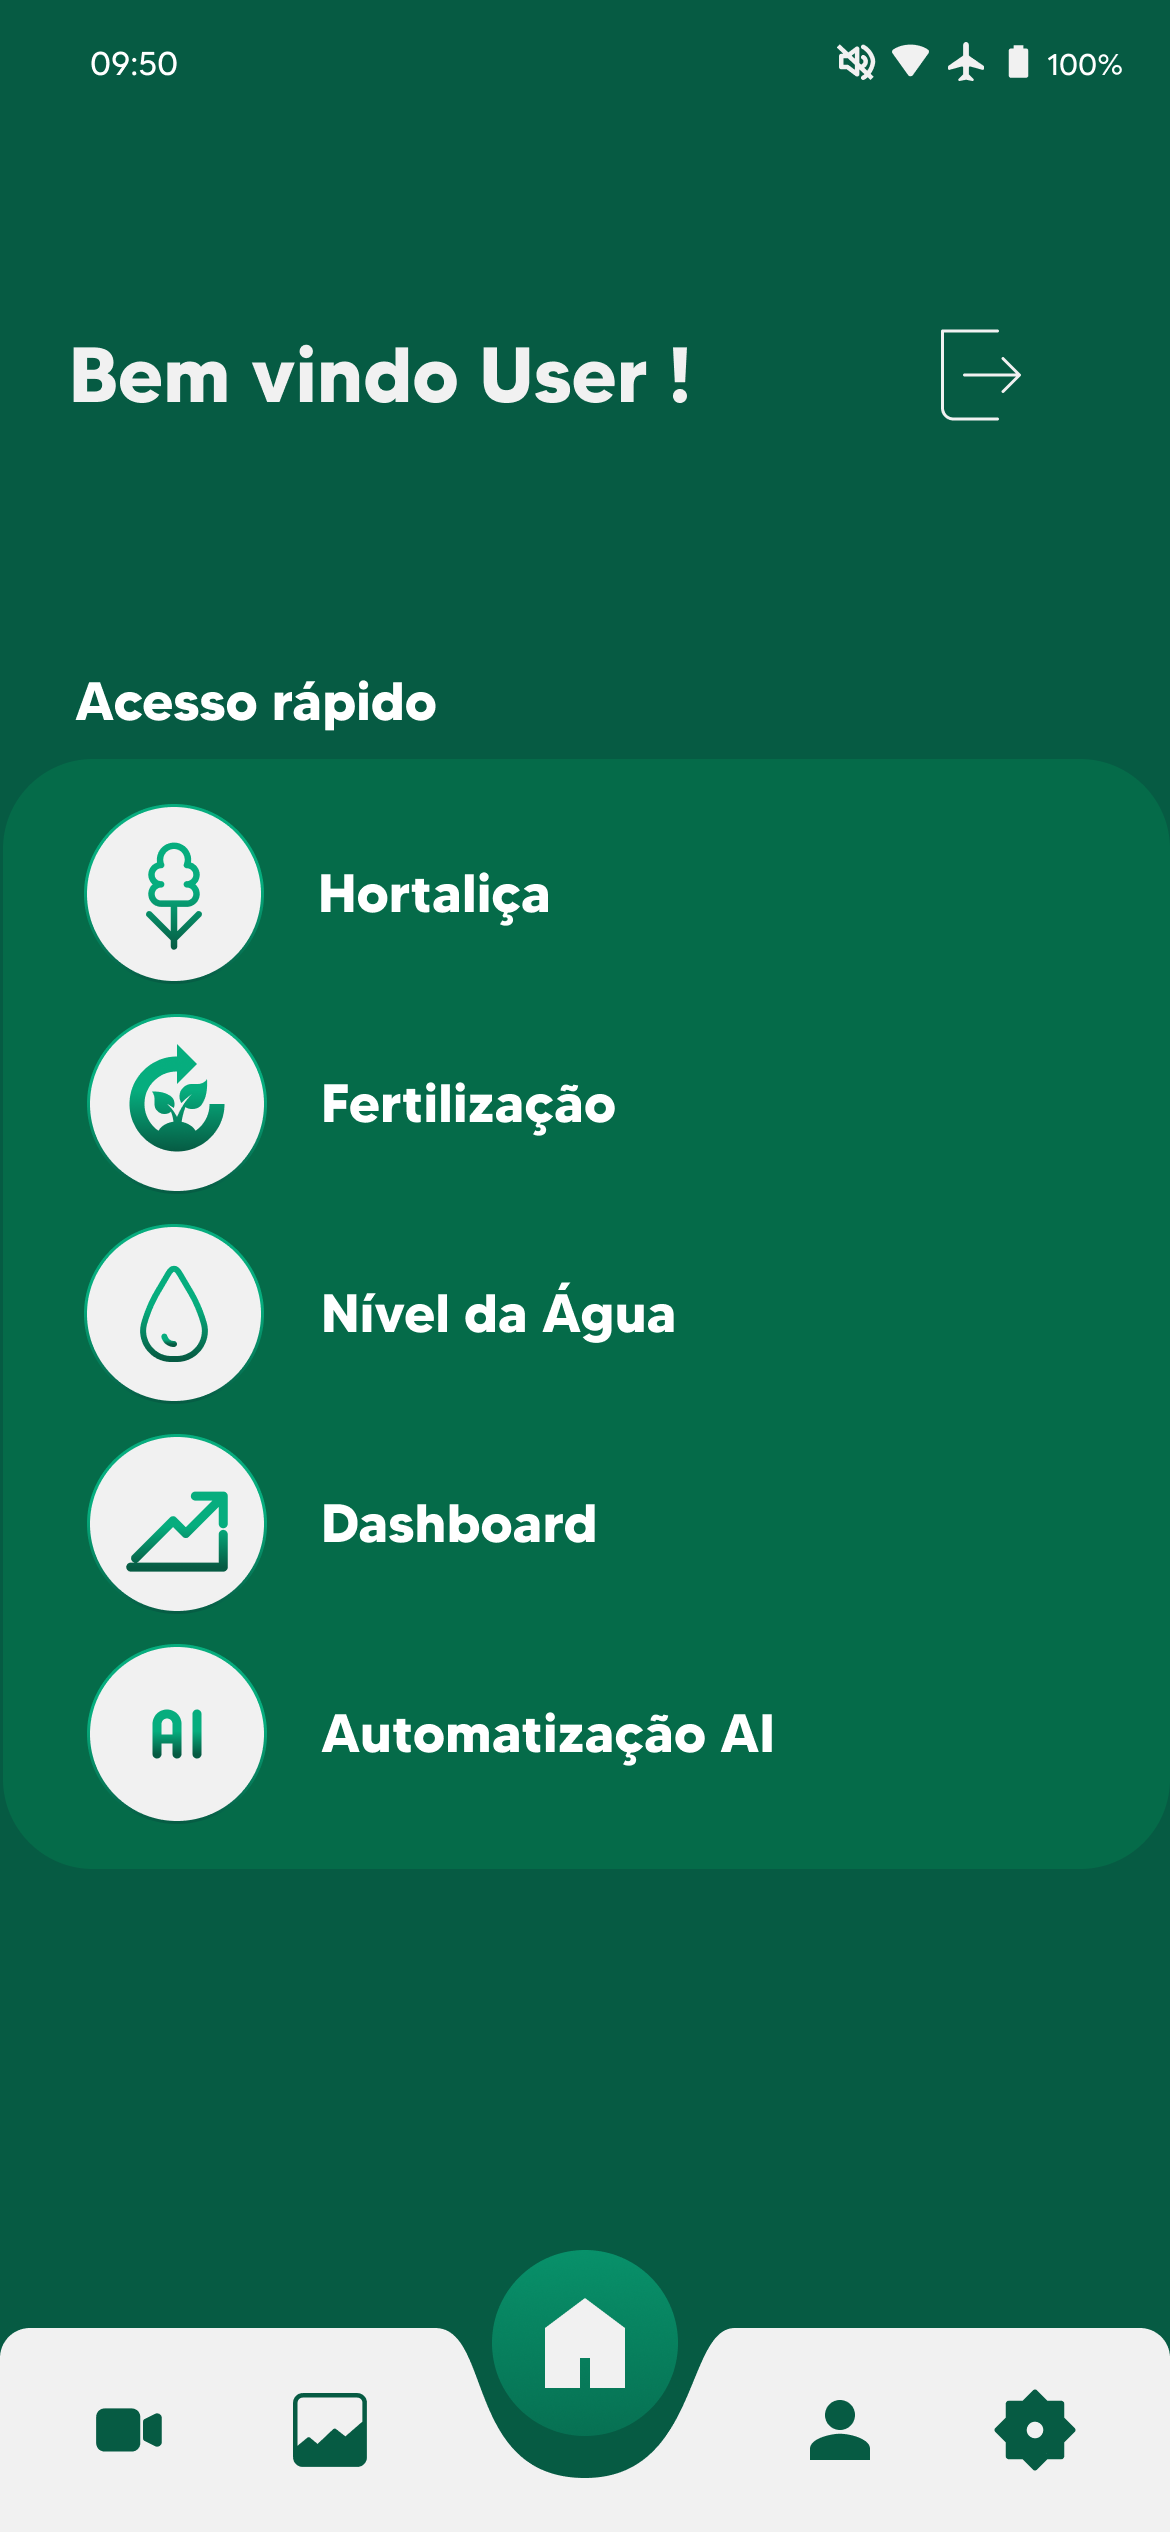
\includegraphics[scale=0.2]{Illustrations/Picture4.png}
\SourceOrNote{Autoria Própria (2024)}
\end{figure}
  
Ao centro da tela de boas-vindas são apresentados ícones de acesso rápido para os menus descritos de câmera em tempo real, hortaliça, fertilização, nível da água, dashboard e automatização AI. Na barra inferior temos o menu interativo do tipo carroussels e interações (da esquerda para a direita) para acesso às telas de câmera em tempo real, dashboards, página inicial, configurações do usuário e configuração do aplicativo. No canto superior direito temos o botão de voltar (que retorna para a tela de login).

\begin{figure}[!h]
\centering
\caption{Tela de dashboards}
\label{fig:picture5}
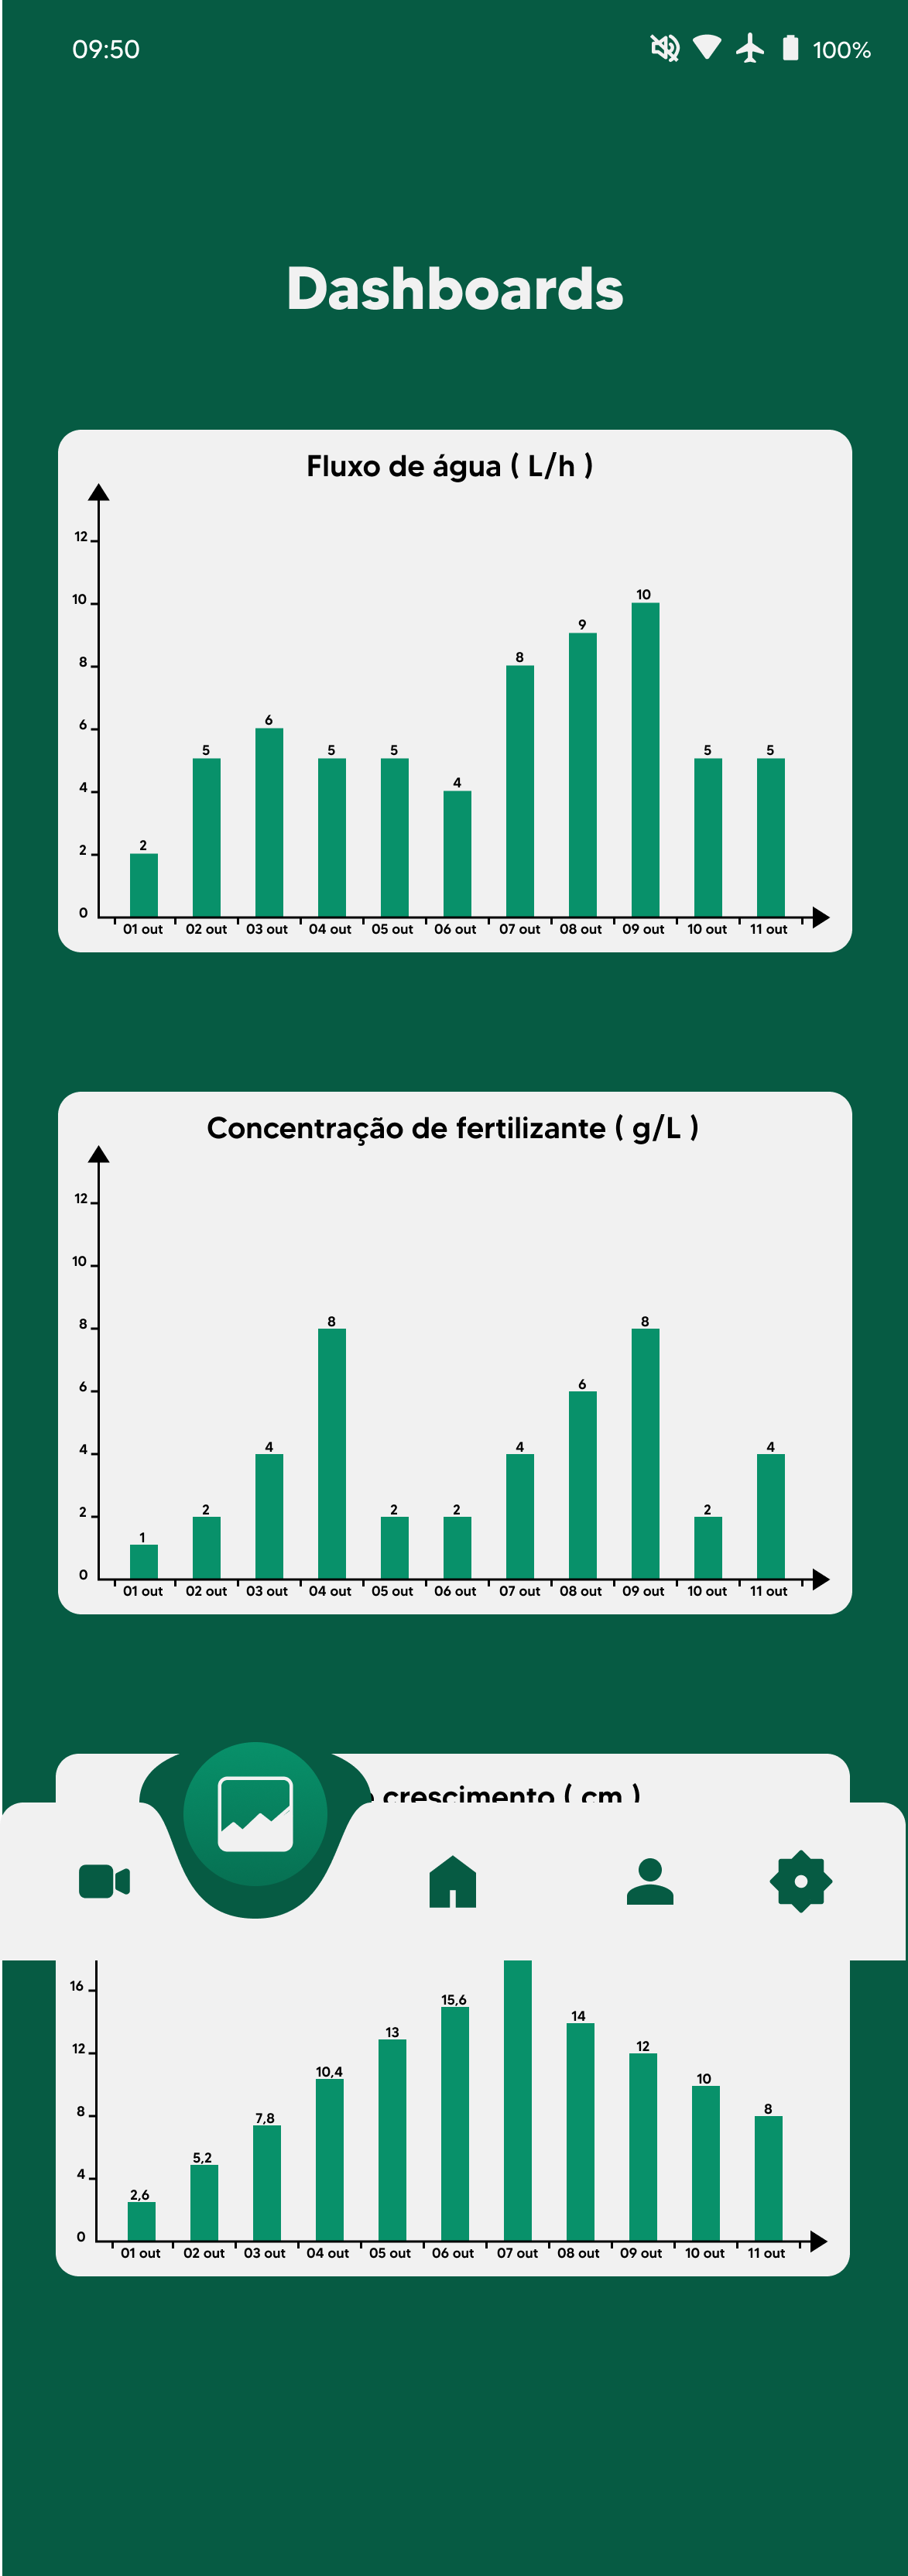
\includegraphics[scale=0.3]{Illustrations/Picture5.png}
\SourceOrNote{Autoria Própria (2024)}
\end{figure}

A tela de dashboards apresenta os dados históricos de fluxo de água, concentração de fertilizante e a taxa de crescimento da(s) cultura(s). A tela tem a opção de rolagem para exibição dos gráficos. Por sua vez, os gráficos são gerados automaticamente com base nos dados obtidos pelos sensores instalados na fazenda vertical.
\clearpage
\begin{figure}[!h]
\centering
\caption{Tela de configurações do aplicativo}
\label{fig:picture6}
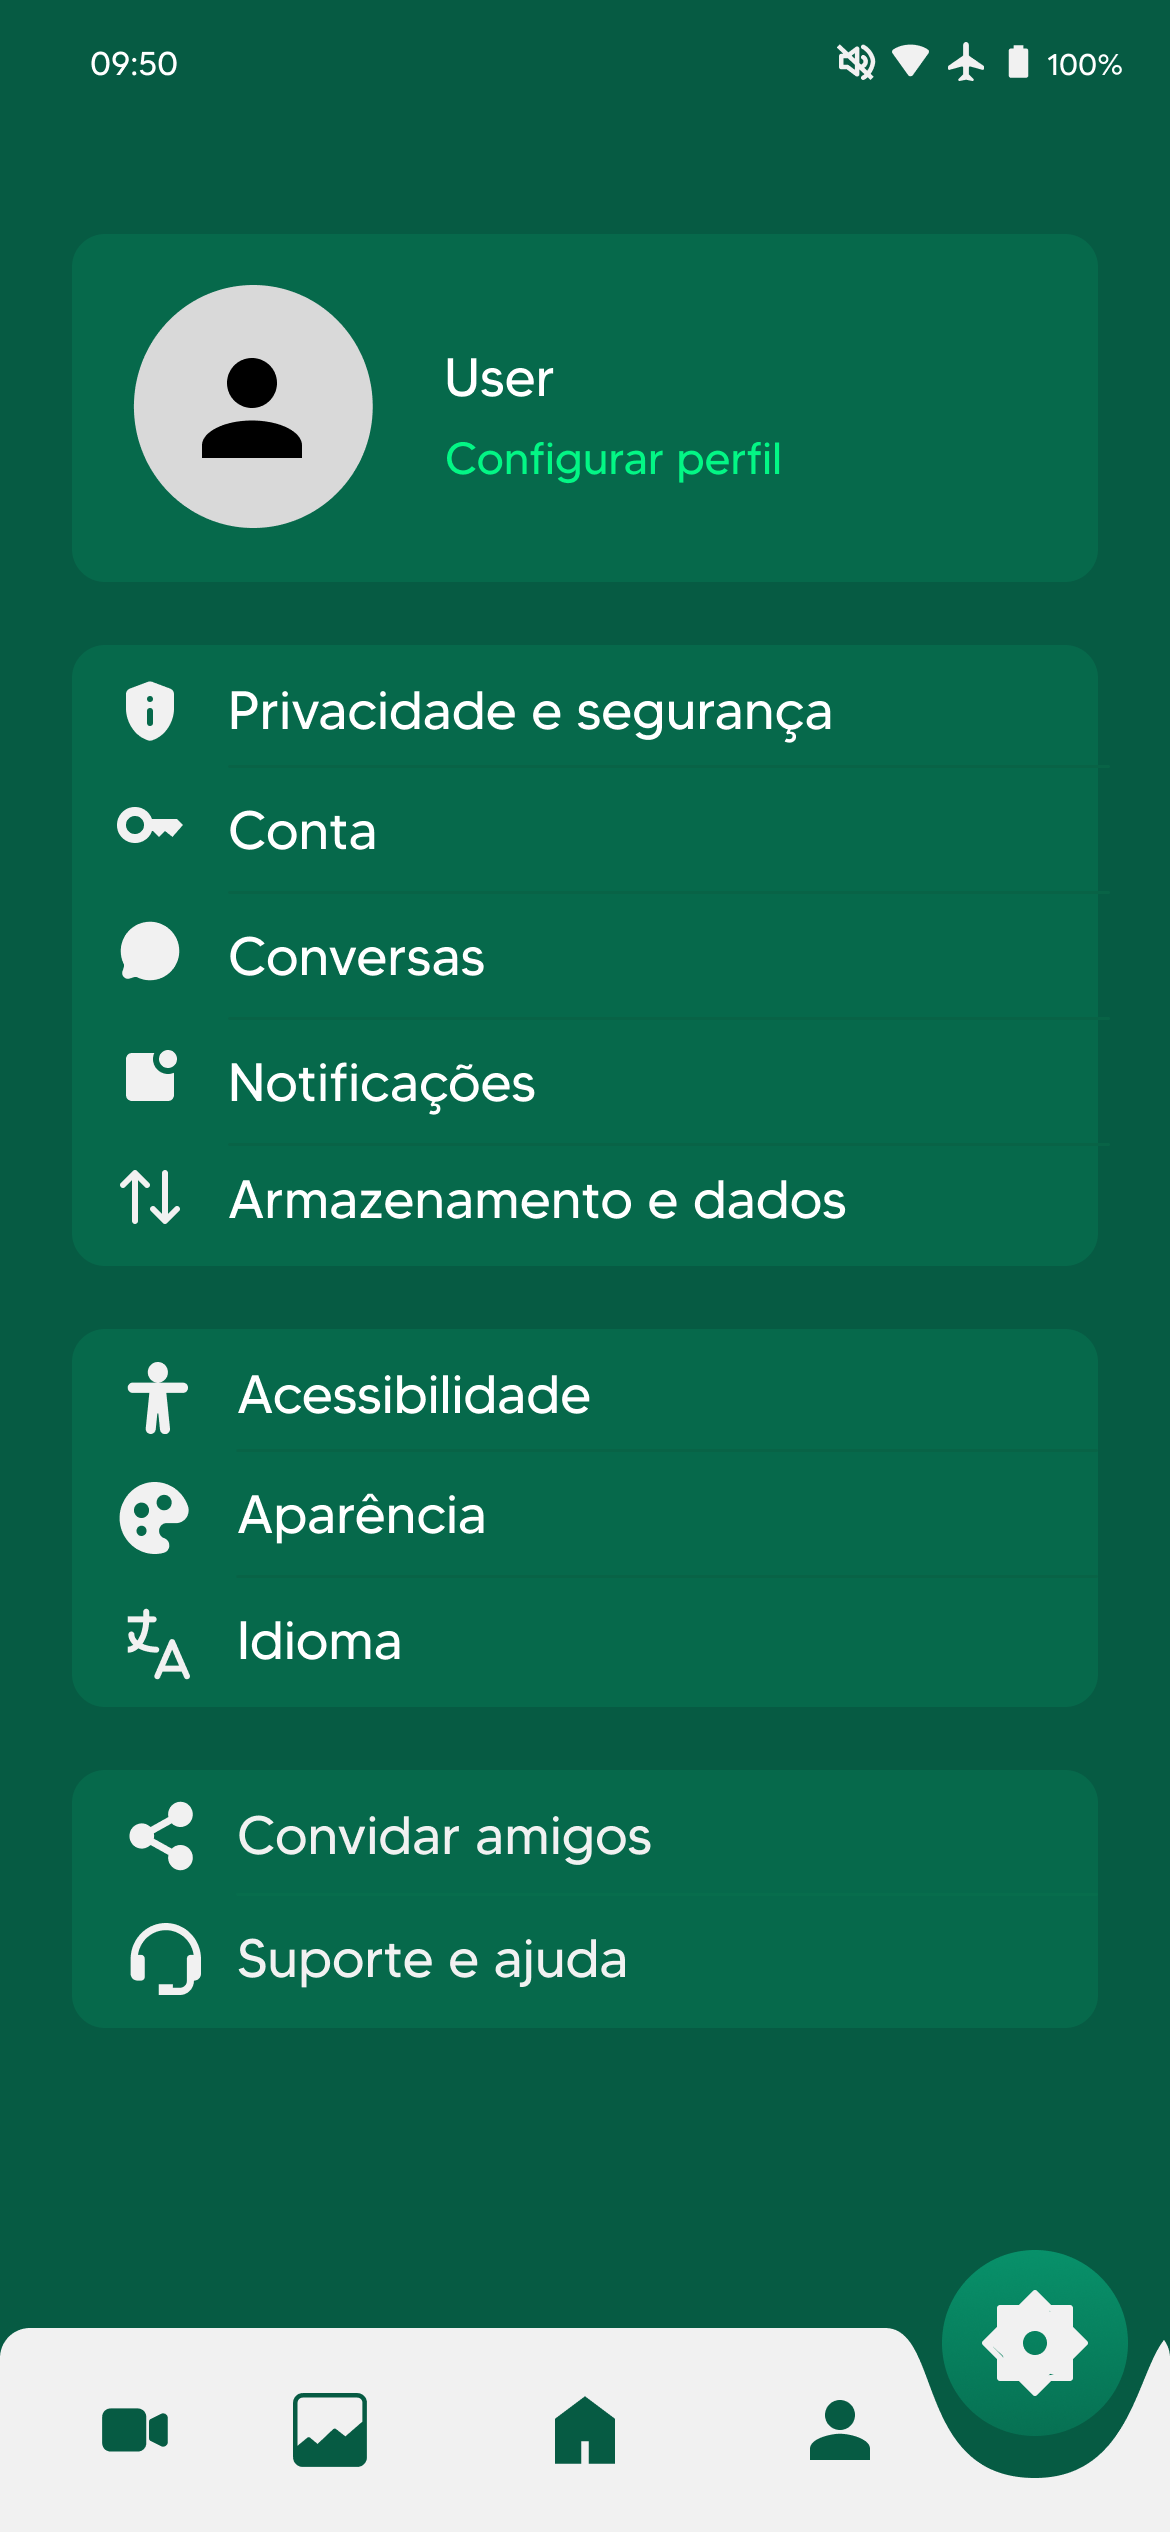
\includegraphics[scale=0.3]{Illustrations/Picture6.png}
\SourceOrNote{Autoria Própria (2024)}
\end{figure}

A tela de configurações do aplicativo é composta da imagem (editável) do usuário com atalho para configurações do perfil e botões de privacidade e segurança, conta, conversas, notificações, armazenamento e dados, acessibilidade, aparência, idioma, convidar amigos e suporte e ajuda.

\begin{figure}[!h]
\centering
\caption{Tela de câmeras}
\label{fig:picture7}
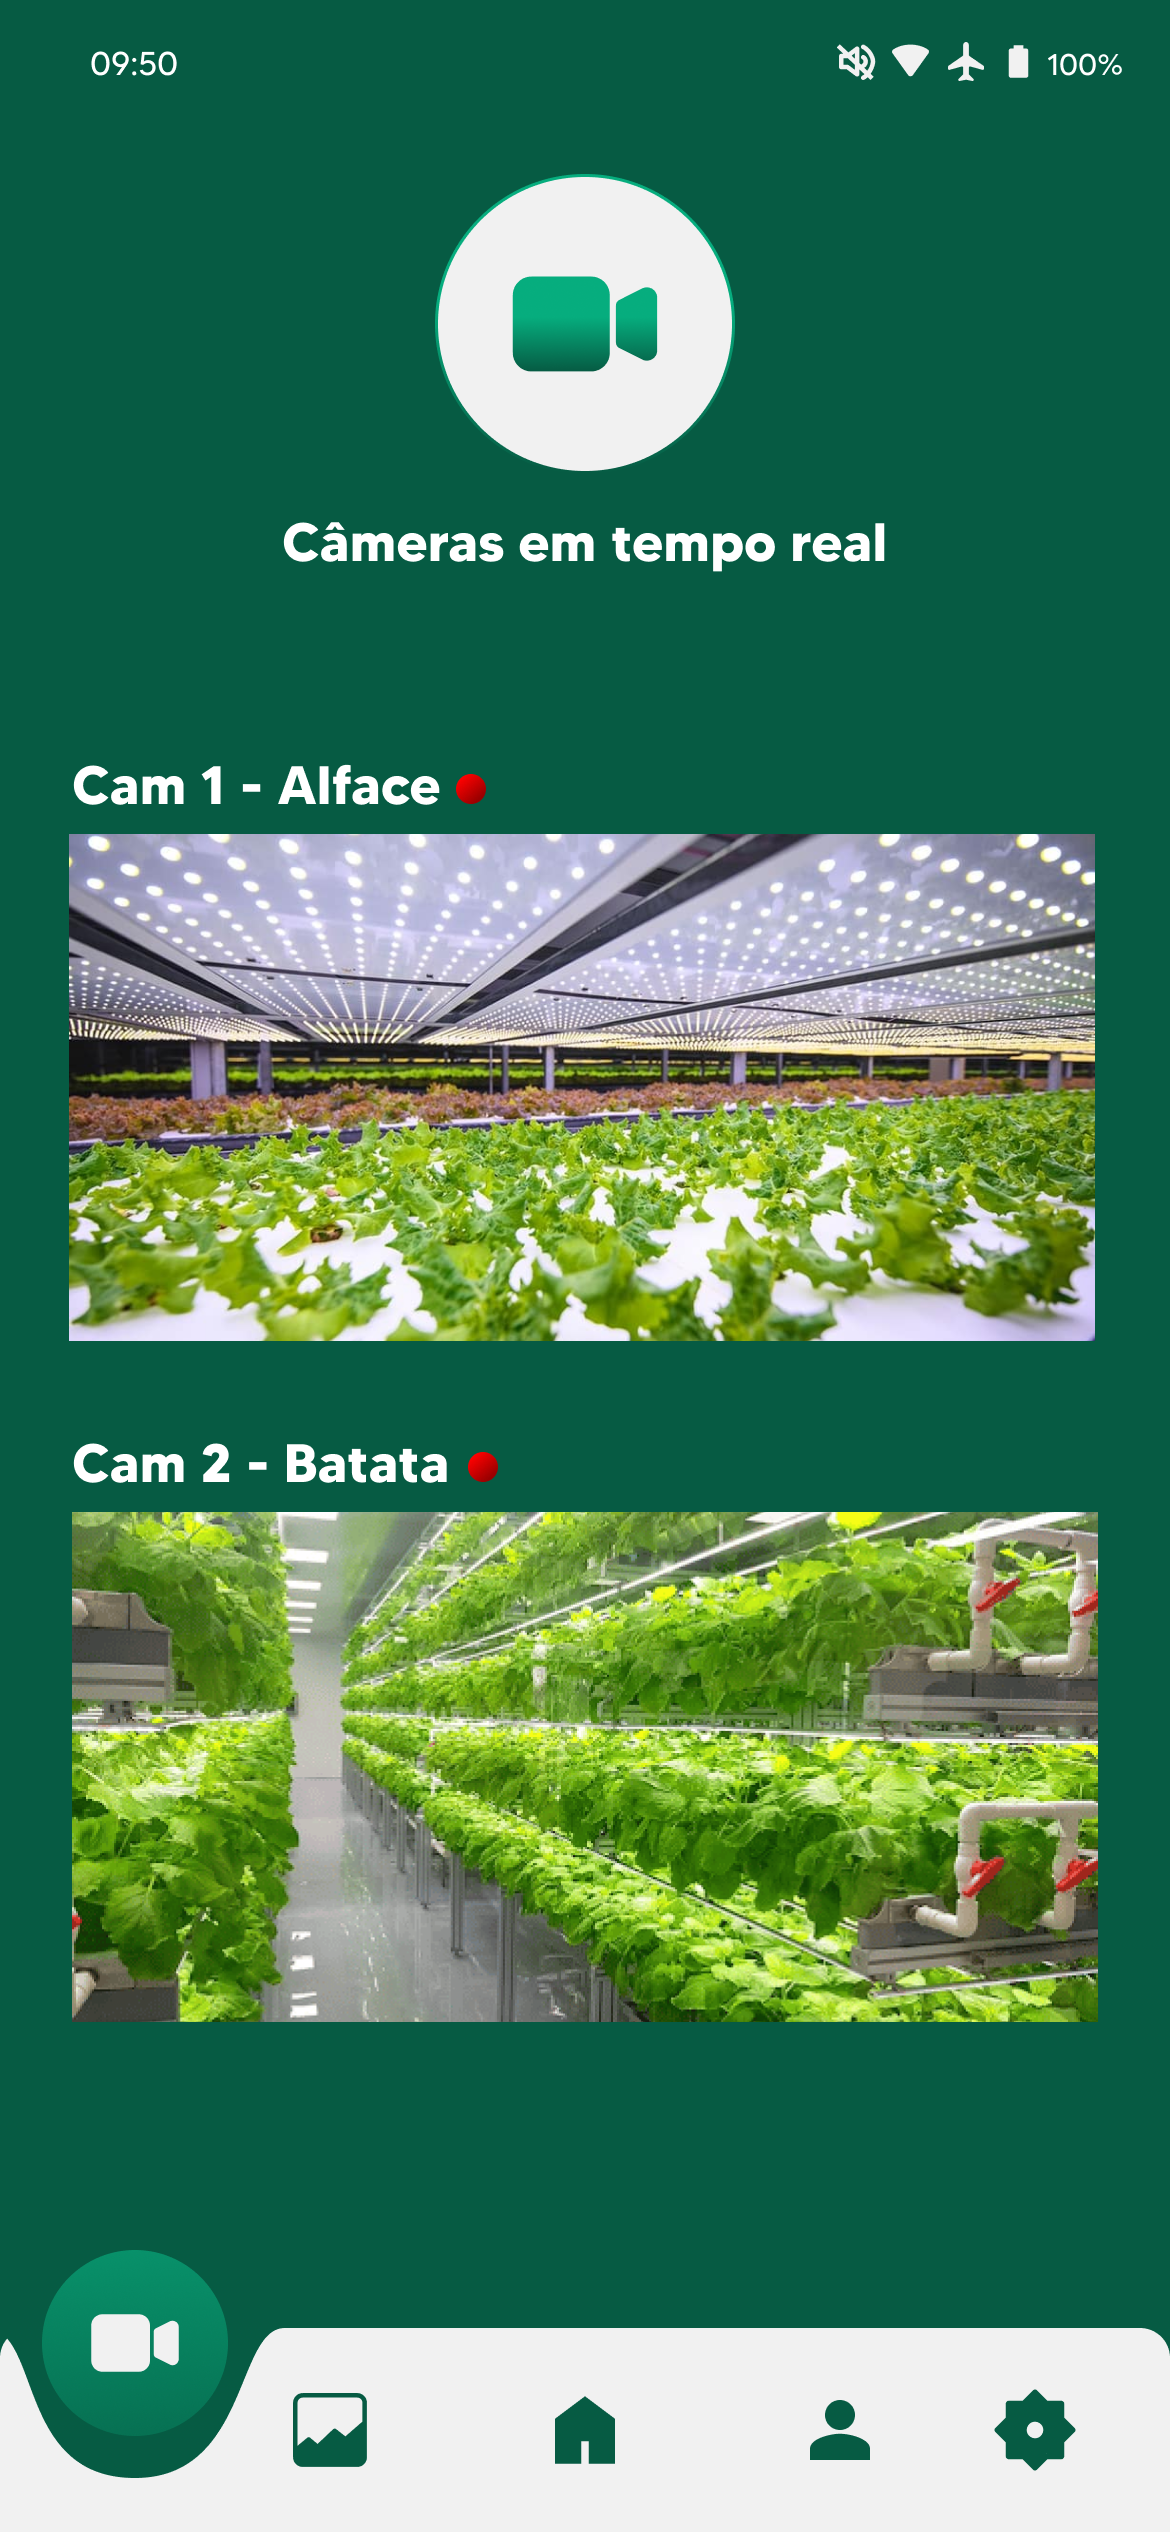
\includegraphics[scale=0.3]{Illustrations/Picture7.png}
\SourceOrNote{Autoria Própria (2024)}
\end{figure}
A tela de câmeras em tempo real contem um íconde decorativo no topo, ao centro. Ela exibe as imagens captadas pela(s) câmera(s) que acompanham a produção da fazenda vertical do usuário. A tela também apresenta a opção de rolagem da página caso tenha mais de uma câmera monitorando a produção da fazenda.

\begin{figure}[!h]
\centering
\caption{Tela de hortaliça}
\label{fig:picture8}

\includegraphics[scale=0.3]{Illustrations/Picture8.png}
\SourceOrNote{Autoria Própria (2024)}
\end{figure}
A tela de hortaliça é composta de um ícone decorativo no topo. Ao centro temos uma lista suspensa onde o usuário deve escolher o tipo de vegetal que será cultivado na fazenda vertical.

\begin{figure}[!h]
\centering
\caption{Tela de fertilização}
\label{fig:picture9}

\includegraphics[scale=0.3]{Illustrations/Picture9.png}
\SourceOrNote{Autoria Própria (2024)}
\end{figure}
A tela de fertilização contém um ícone decorativo centralizado, acima. Ao centro da tela temos um campo onde o usuário deverá digitar a concentração do fertilizante em gramas por litro.
\begin{figure}[!h]
\centering
\caption{Tela de nível da água}
\label{fig:picture10}
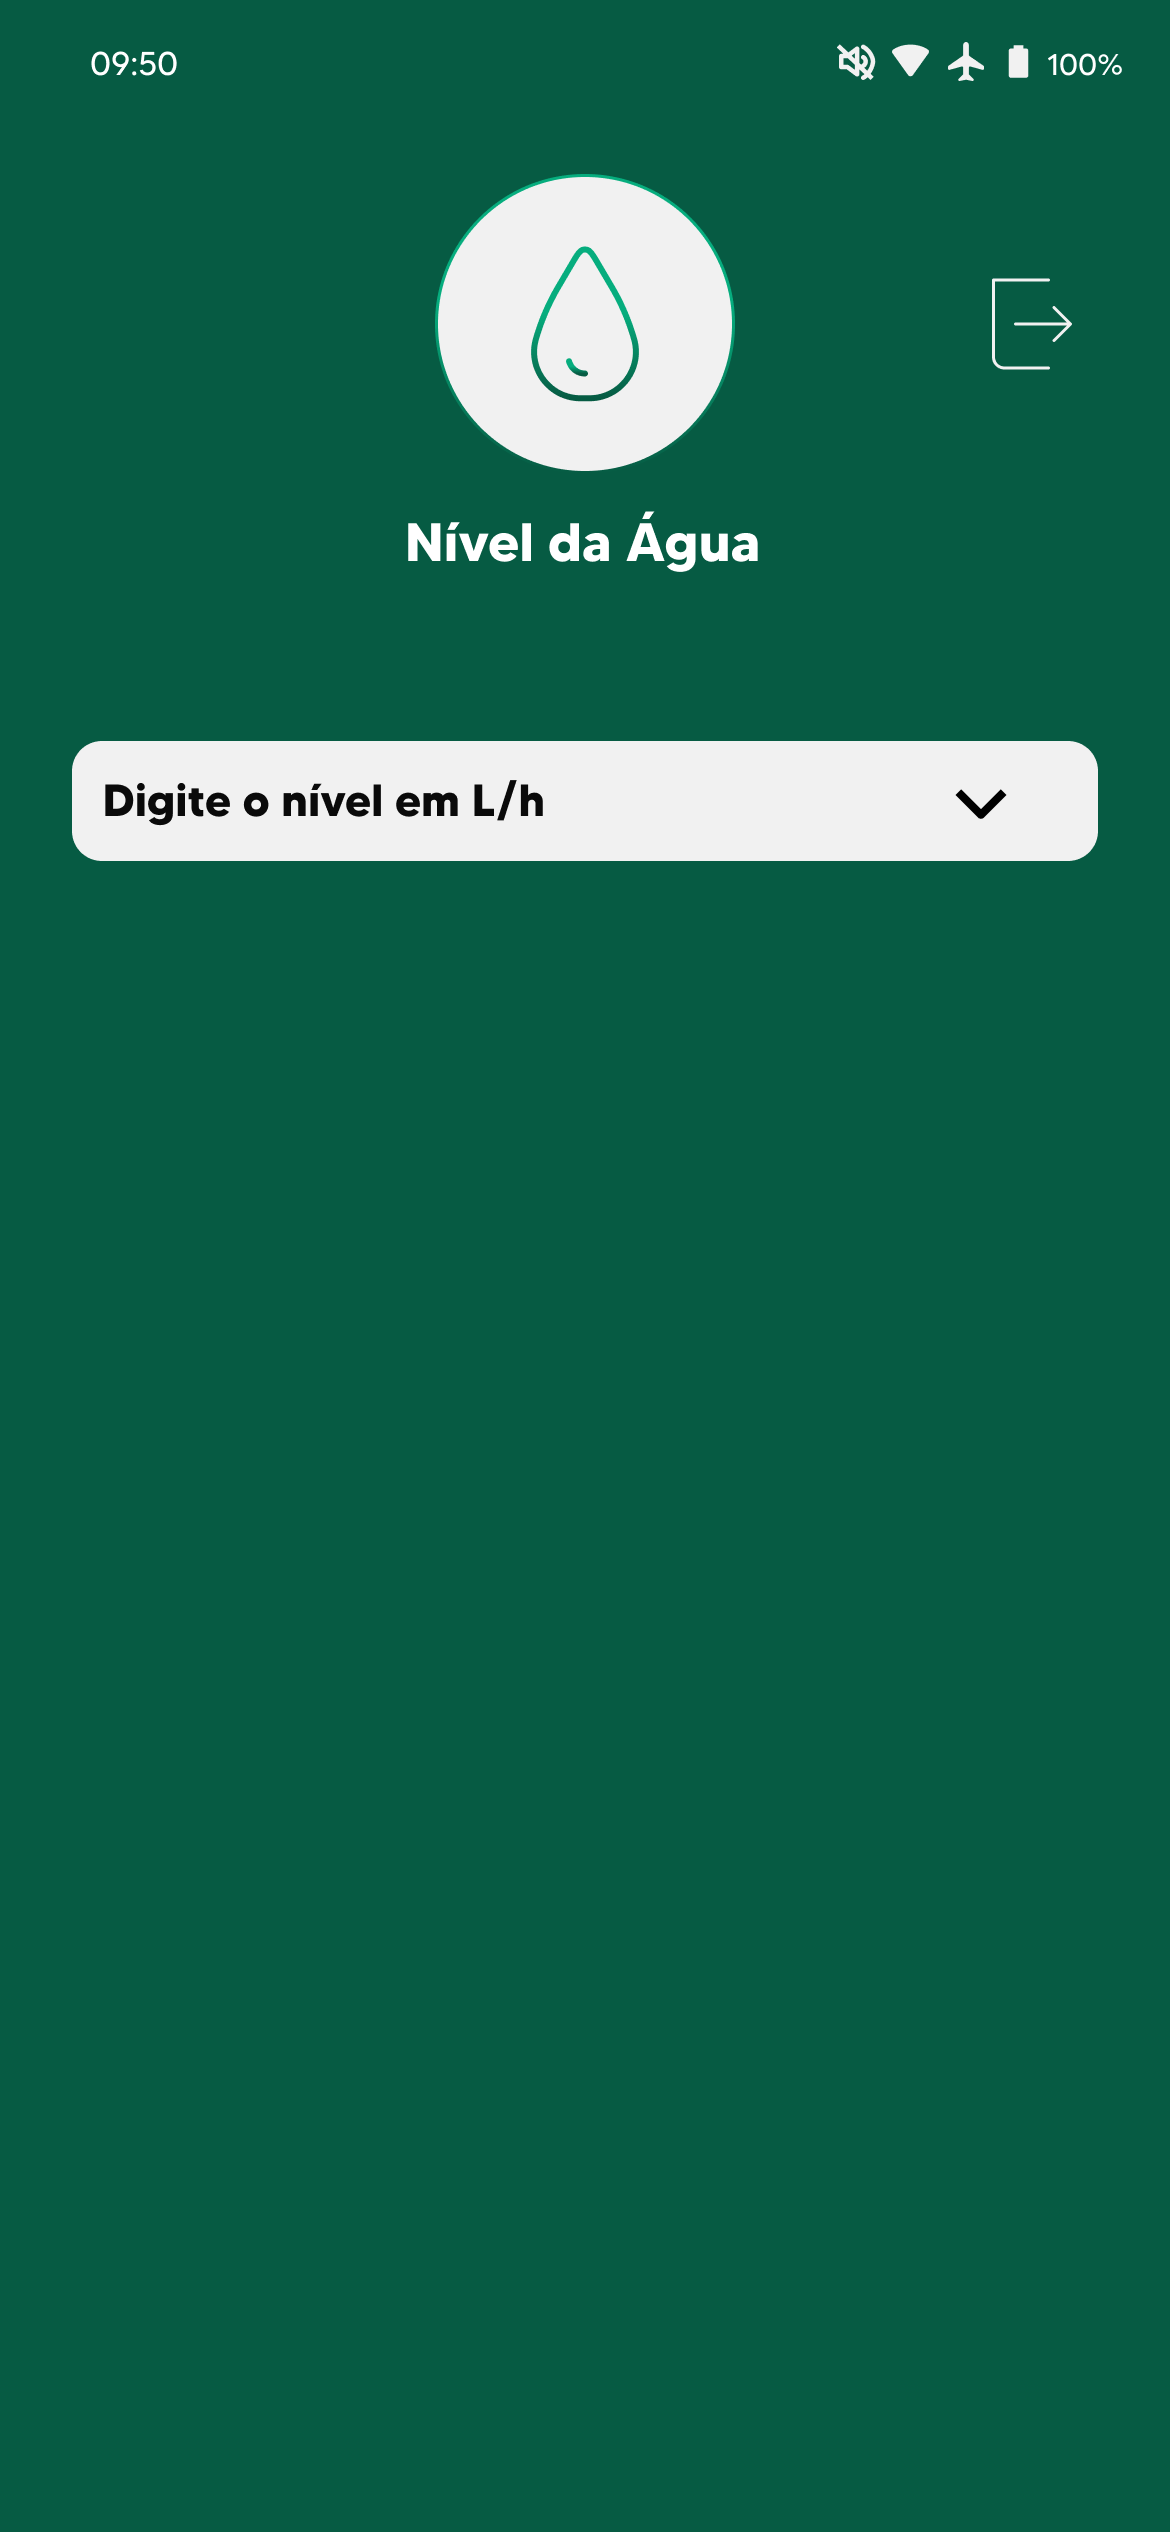
\includegraphics[scale=0.3]{Illustrations/Picture10.png}
\SourceOrNote{Autoria Própria (2024)}
\end{figure}
A tela de nível da água contém um ícone decorativo centralizado no topo. Nesta tela o usuário deverá digitar a pressão da água (em litros por hora) que passa pelo sistema de fazenda vertical.
\clearpage
\begin{figure}[!h]
\centering
\caption{Tela de automatização AI}
\label{fig:picture11}

\includegraphics[scale=0.2]{Illustrations/Picture11.png}
\SourceOrNote{Autoria Própria (2024)}
\end{figure}
A tela de automatização AI permite que o usuário escolha se deseja que a rede neural tenha total controle da fazenda vertical e sua produção. Esta tela também oferece a opção de o usuário controlar pessoalmente alguns parâmetros (controle semi-autônomo) ou controlar todas as configurações (controle manual).
            
\subsection*{DIAGRAMA DE BANCO DE DADOS}

A modelagem do banco de dados foi realizada no software Brmodelo. A modelagem de dados define como o sistema vai trabalhar o fluxo de dados e como estes dados serão utilizados. No contexto deste estudo, os dados desempenham um papel central no processo de tomada de decisão, seja por meio de algoritmos de inteligência artificial, seja por intervenção direta do usuário.

\subsection*{1. Modelo conceitual}

O modelo conceitual foi desenvolvido para representar o banco de dados com foco em entidades, atributos e os relacionamentos entre eles. A seguir é apresentada a estrutura conceitual do banco de dados proposto.

\clearpage
\begin{figure}[!h]
\centering
\caption{Modelo conceitual}
\label{fig:picture14}
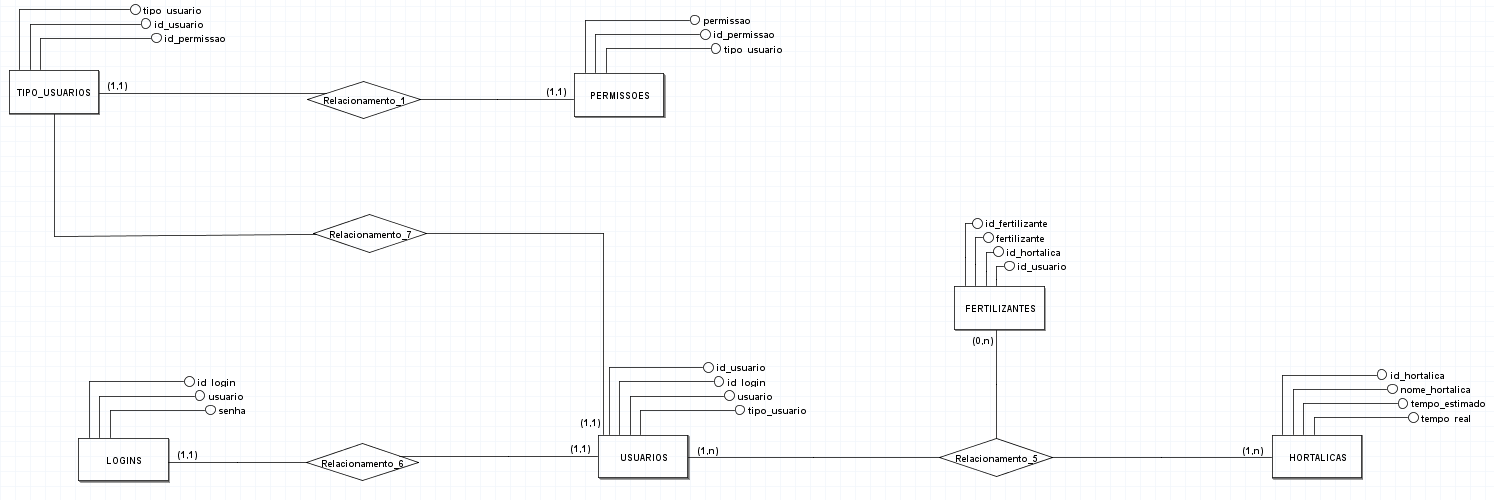
\includegraphics[scale=0.4]{Illustrations/modelo conceitual.png}
\SourceOrNote{Autoria Própria (2024)}
\end{figure}

Foram mapeadas seis entidades (colunas) diferentes, vinte e um atributos e quatro relacionamentos.

\subsection*{2. Modelo lógico}

O modelo lógico detalha o banco de dados em termos de atributos específicos, incluindo tipo de dado, obrigatoriedade e unicidade. 

\begin{figure}[!h]
\centering
\caption{Modelo clógico}
\label{fig:picture15}
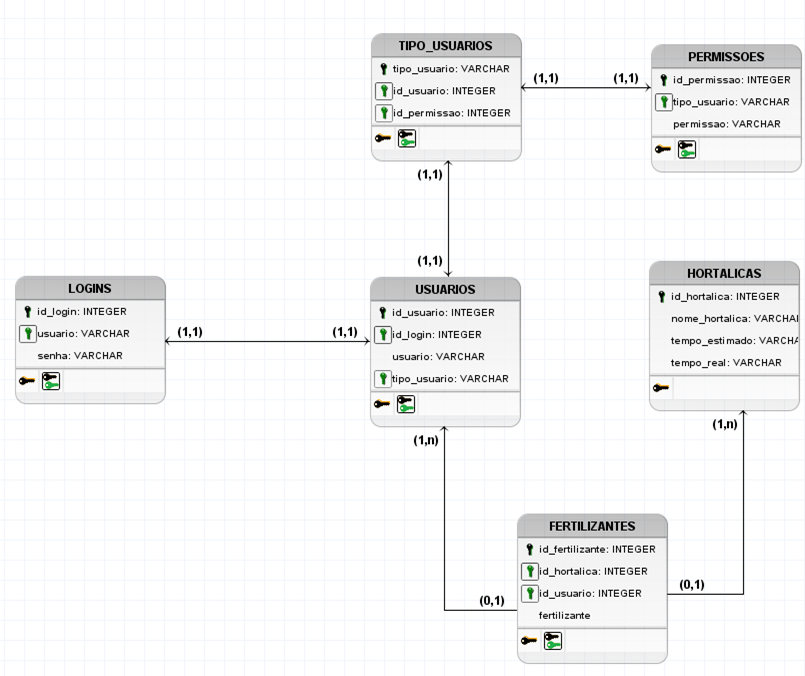
\includegraphics[scale=0.8]{Illustrations/modelo logico.png}
\SourceOrNote{Autoria Própria (2024)}
\end{figure}

Nesta fase foram identificadas seis chaves primárias e oito chaves estrangeiras. O modelo inclui ainda dez atributos do tipo INTEGER e onze atributos do tipo VARCHAR que representam dados numéricos e textuais, respectivamente. Realizamos uma revisão para garantir que todas as entidades tivessem chaves primárias entre seus atributos, garantindo a unicidade do banco de dados. Além disso, o sistema contará com diversas chaves estrangeiras que realizem corretamente o relacionamento entre as entidades envolvidas.

\subsection*{DIAGRAMA DE SISTEMA}

A diagramação do sistema foi realizada considerando pontos-chave para a estrutura do software. Primeiramente, à partir do celular do usuário (a), os dados serão enviados à um roteador conectado à internet (b). Paralelamente na fazenda vertical, o(s) sensor(es) conectado(s) por Arduino (c) enviarão seus resultados também para internet via roteador. Na sequência os dados serão armazenados (d) em nuvem utilizando o sistema Oracle Cloud (f). Utilizando o sistema GenAI Oracle os dados são analisados (e) e uma resposta é enviada ao celular do usuário, apresentando os valores ideais de operação identificados pelo algoritmo. Além disso, também conectado ao Oracle Cloud teremos um PC emitindo relatórios em tempo real sobre o banco de dados e informações relevantes sobre o status da operação (g).

\begin{figure}[!h]
\centering
\caption{Diagrama de sistema}
\label{fig:picture16}
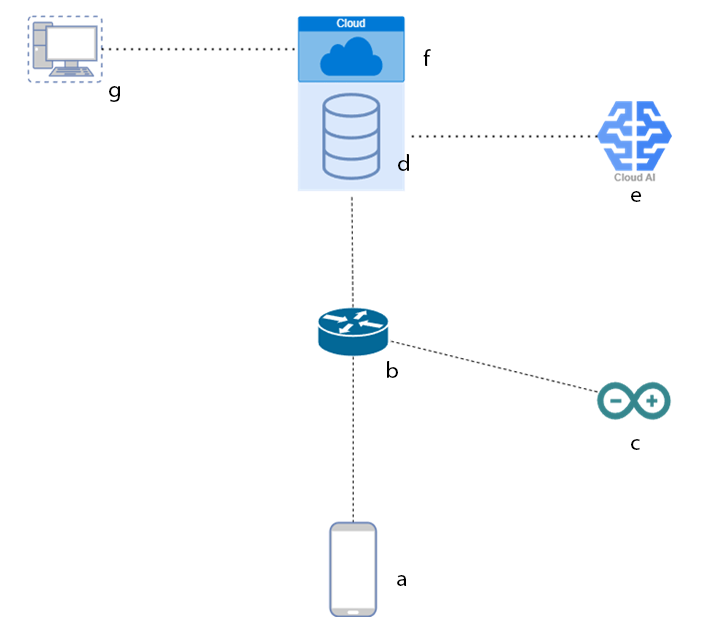
\includegraphics[scale=0.8]{Illustrations/diagrama de sistema 2.png}
\SourceOrNote{Autoria Própria (2024)}
\end{figure}
Esta é uma etapa crítica pois uma das bases do trabalho é a utilização da rede neural para o desenvolvimento do projeto. Além disso o sistema de armazenamento em nuvem e backup garantem a integridade dos dados.
\subsection*{ANÁLISE DO PROJETO (CANVAS)}

A análise do projeto foi realizada por meio do Canvas disponível no site do Sebrae. A avaliação foi realizada levando em consideração os dados levantados no presente projeto e aspectos potenciais da proposta.

\clearpage
\begin{figure}[!h]
\centering
\caption{Diagrama de sistema}
\label{fig:picture17}
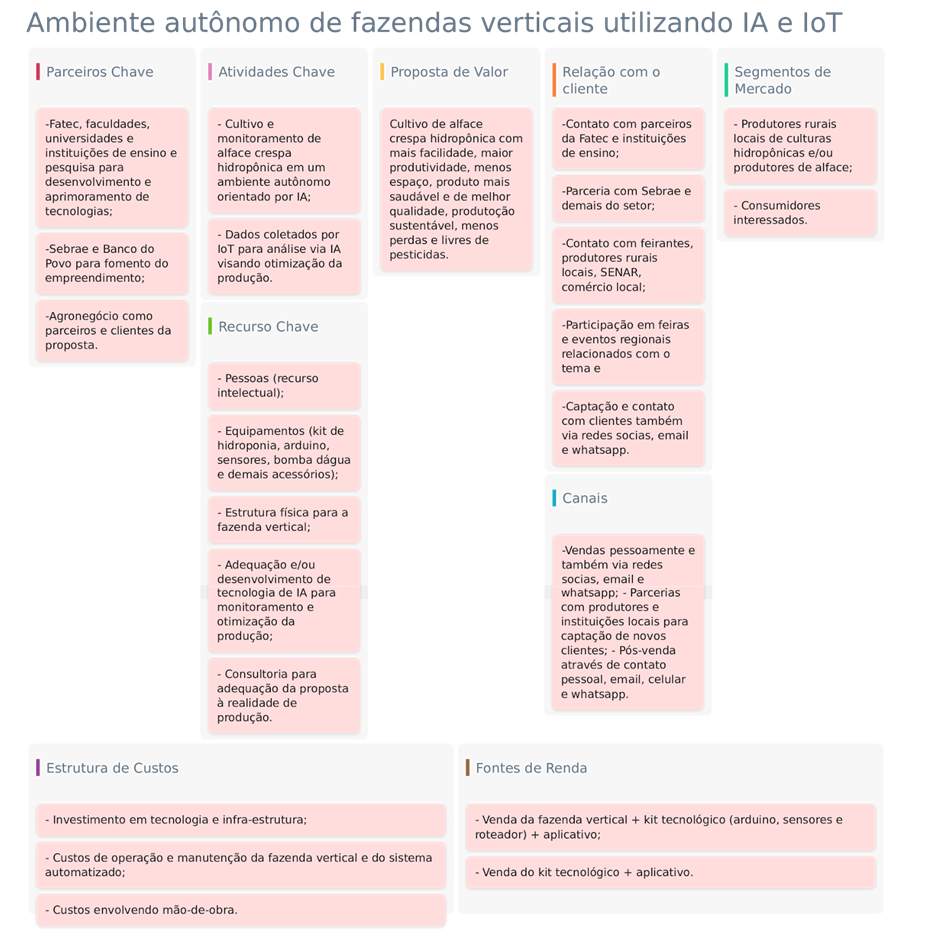
\includegraphics[scale=0.8]{Illustrations/CANVAS.png}
\SourceOrNote{Autoria Própria (2024)}
\end{figure}

Com o Canvas é possível observar o caráter empreendedor do projeto. Além disso observamos diversas oportunidades e pontos de melhoria que impactam na viabilidade do projeto como empreendimento.

\subsection*{PLATAFORMA WEB (APEX)}

O sistema proposto foi elaborado na plataforma web em um sistema low code. Todo o sistema é responsivo, podendo ser exibido tanto em smartphones quanto em tablets ou computadores. A plataforma apresenta por padrão um banco de dados em nuvem, garantindo assim a integridade dos dados. 
\clearpage
\begin{figure}[!h]
\centering
\caption{Tela de login}
\label{fig:picture18}
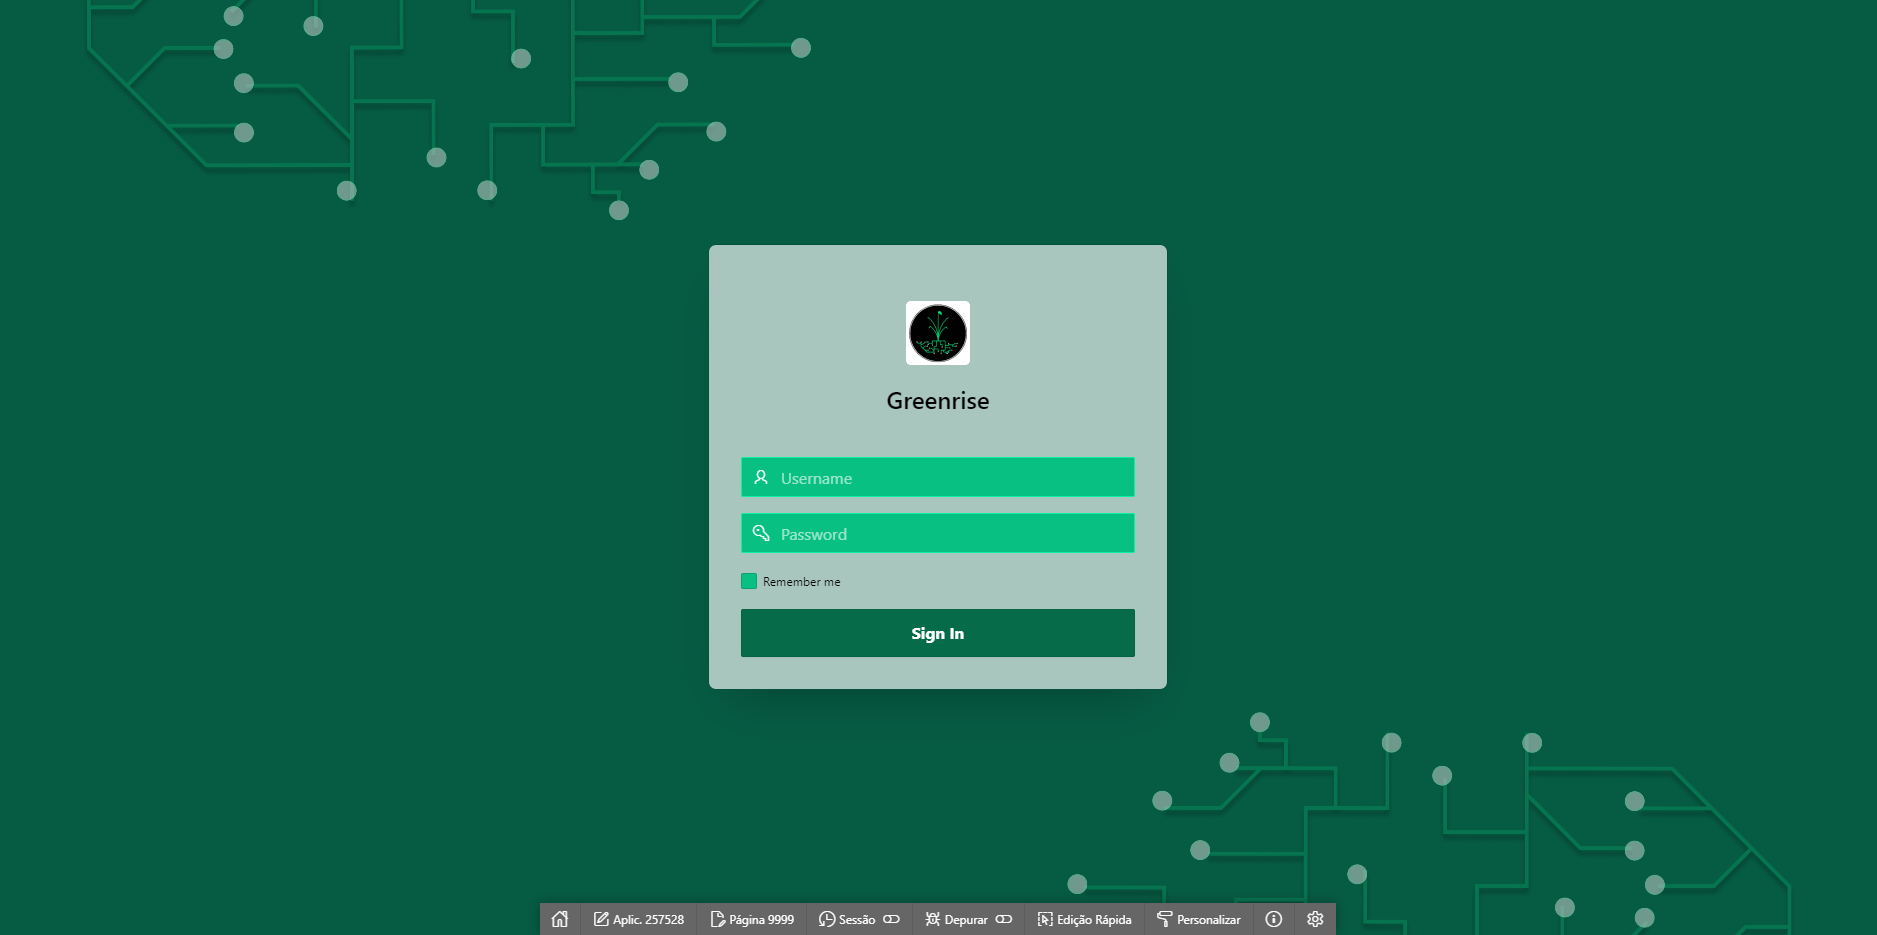
\includegraphics[scale=0.2]{Illustrations/Tela_login.png}
\SourceOrNote{Autoria Própria (2024)}
\end{figure}
Seguindo as premissas pré-estabelecidas o sistema foi elaborado com uma tela de login (onde o usuário preenche com seu nome e senha) para acesso ao sistema. Esta também é uma forma de garantir a segurança do acesso ao sistema.
\begin{figure}[!h]
\centering
\caption{Tela inicial}
\label{fig:picture19}
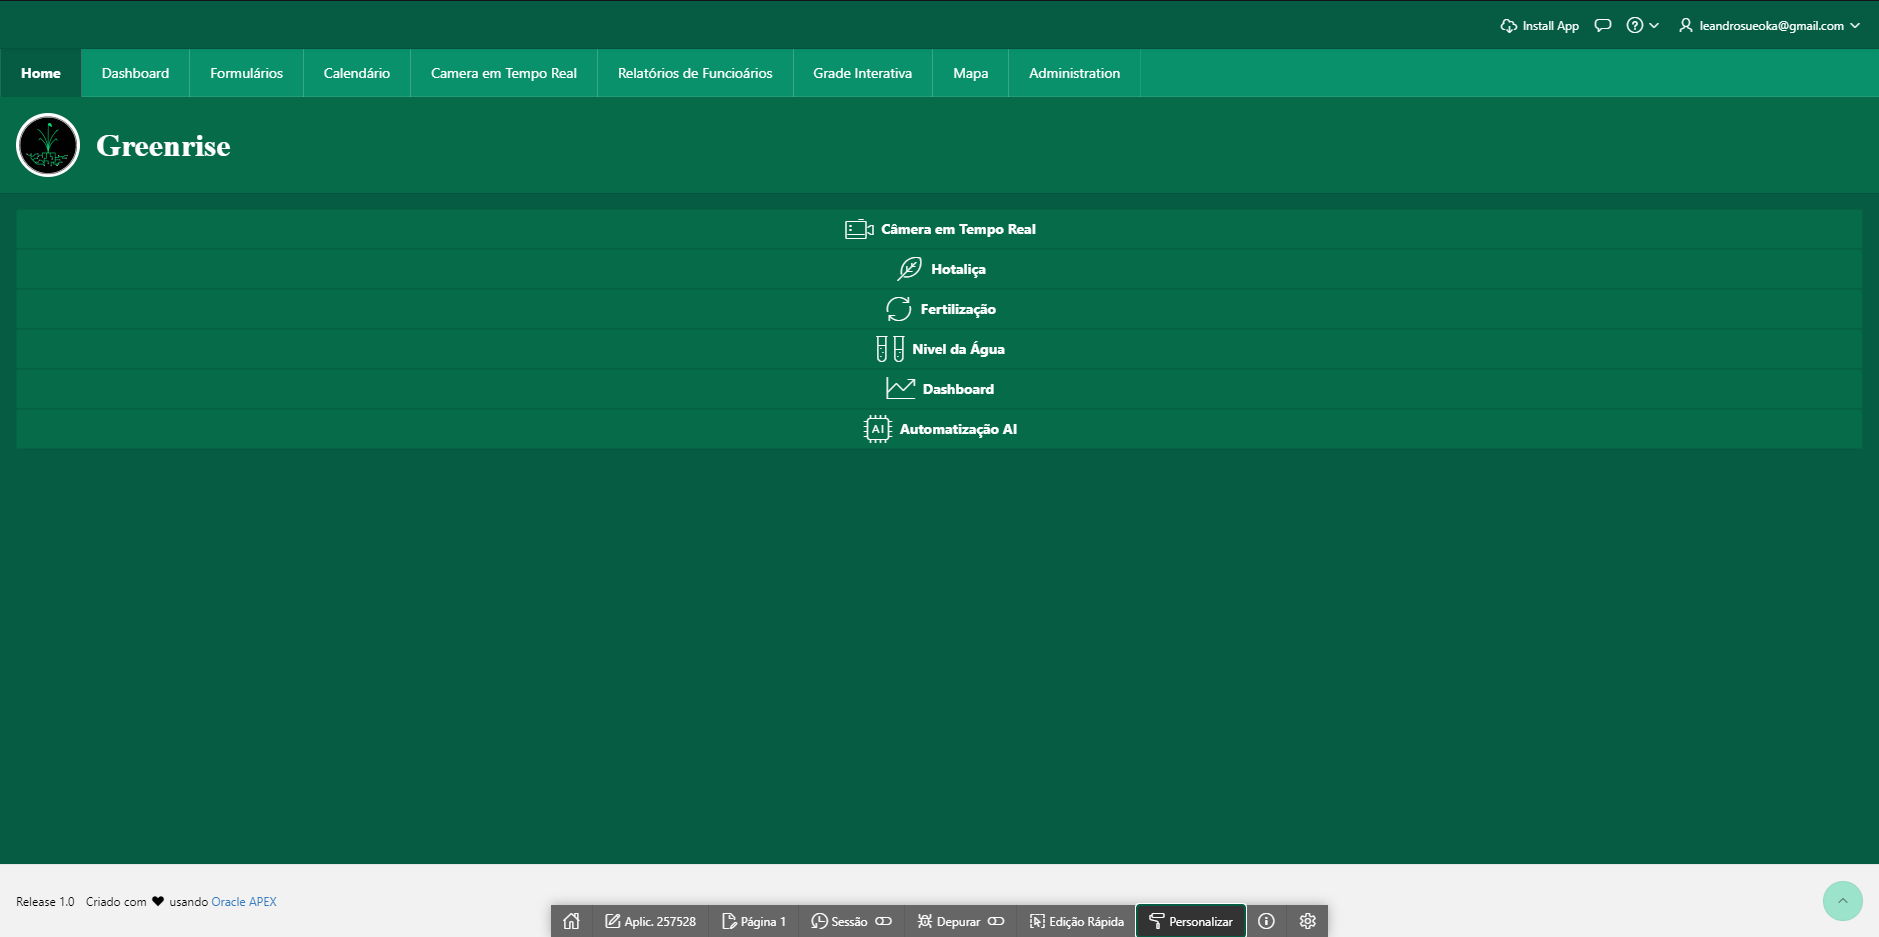
\includegraphics[scale=0.2]{Illustrations/Tela_home.png}
\SourceOrNote{Autoria Própria (2024)}
\end{figure}

Na tela inicial são apresentados os dados cadastrados (tipo de hortaliça, fertilizante, concentração e fluxo de água). Na barra superior temos o menu onde é possível navegar pelas telas do sistema.

\begin{figure}[!h]
\centering
\caption{Tela de dashboards}
\label{fig:picture20}
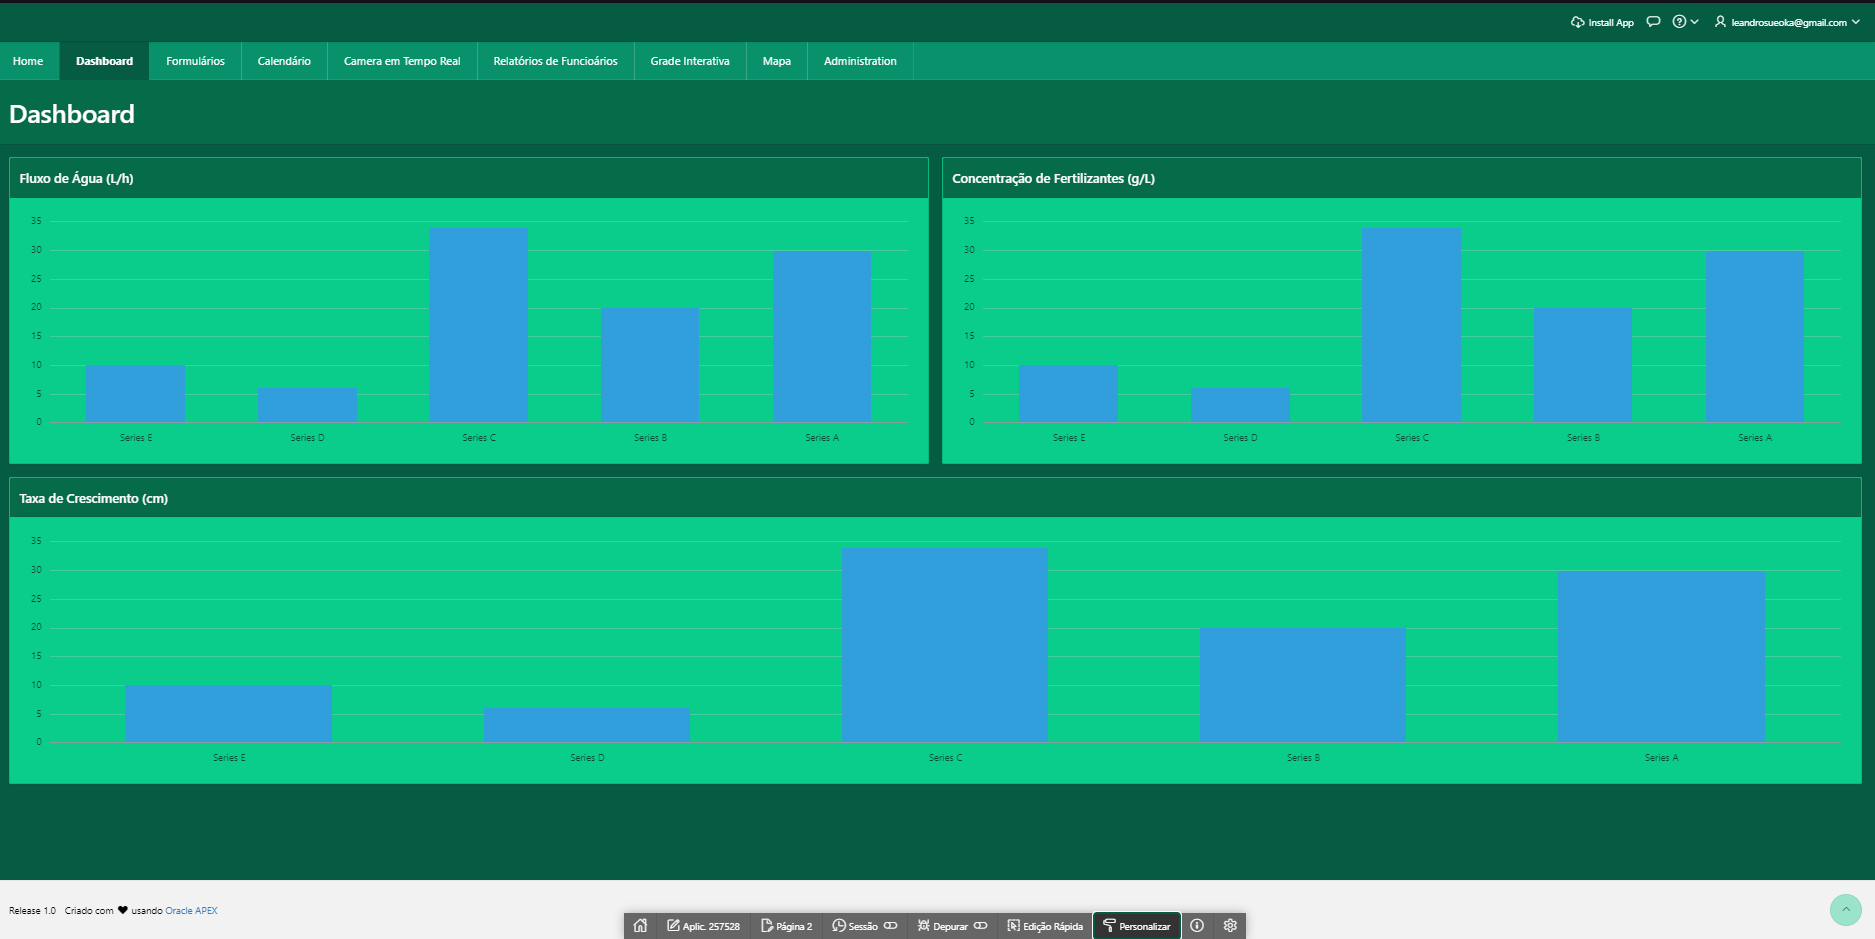
\includegraphics[scale=0.2]{Illustrations/Tela_dashboard.png}
\SourceOrNote{Autoria Própria (2024)}
\end{figure}

Temos uma tela de dashboards com os indicadores apresentando dados históricos de taxa de crescimento, fluxo de água e concentração do fertilizante. São gráficos baseados em Oracle Jet, personalizáveis pelo adminitrador do sistema.

\begin{figure}[!h]
\centering
\caption{Tela de relatórios}
\label{fig:picture21}
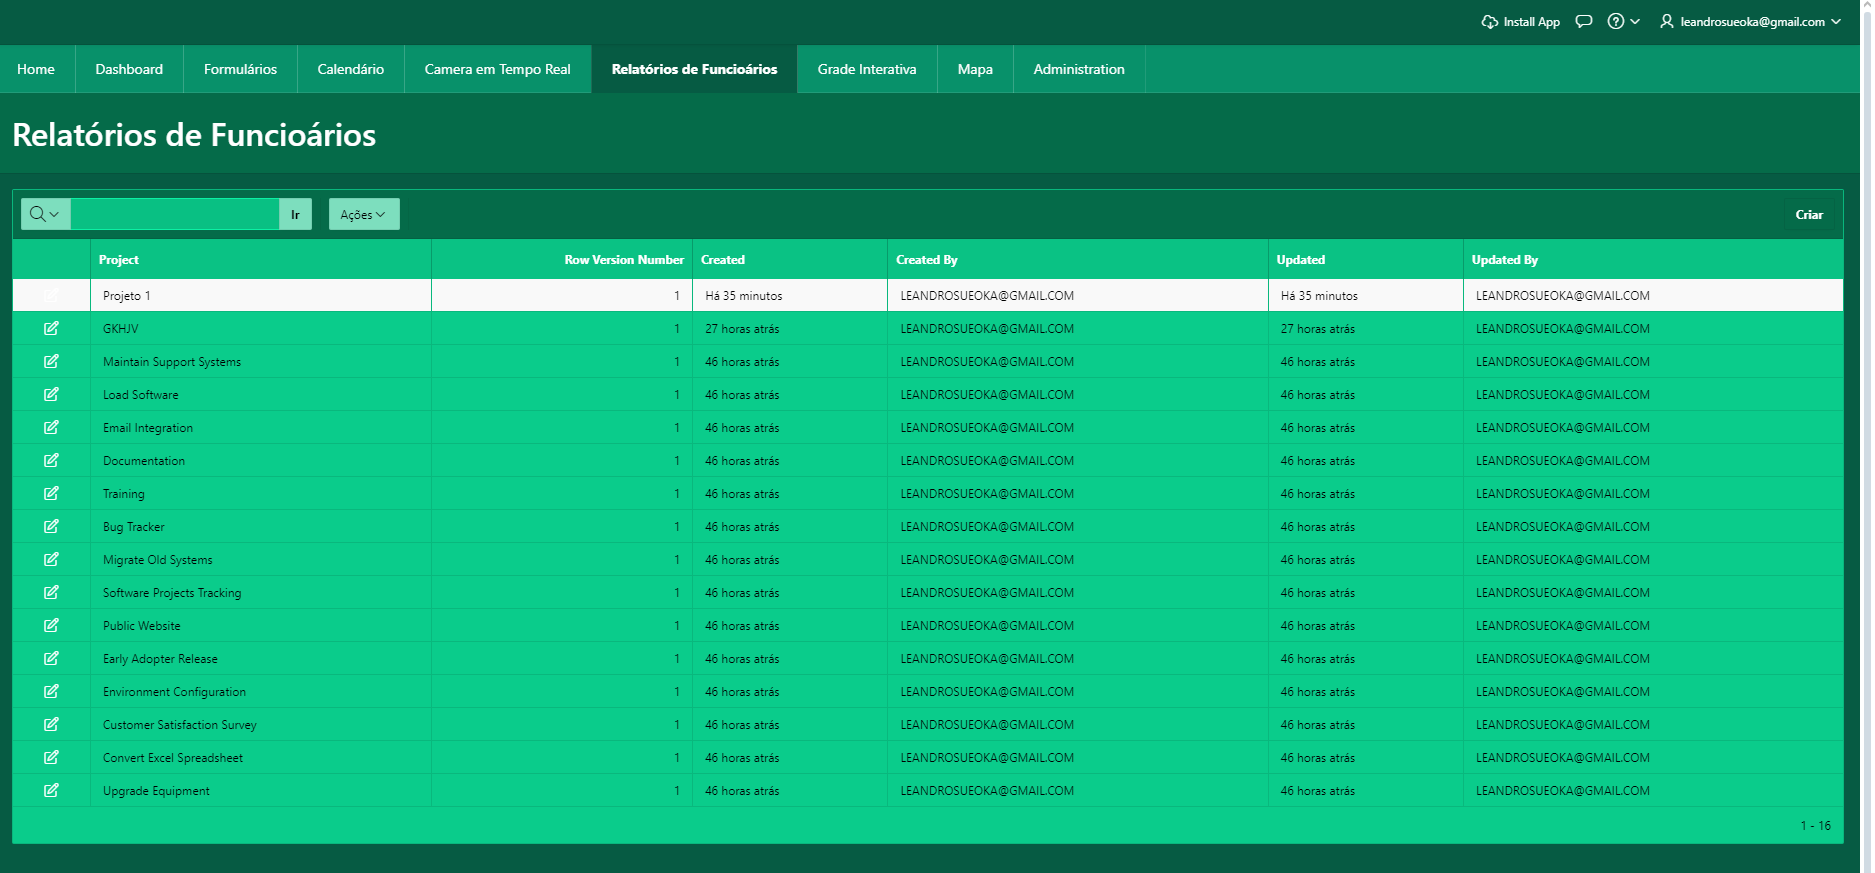
\includegraphics[scale=0.2]{Illustrations/Tela_relatorios_func.png}
\SourceOrNote{Autoria Própria (2024)}
\end{figure}

Temos uma tela de relatórios onde o usuário pode extrair informações mais detalhadas do banco de dados do sistema. Existe um campo de busca onde é possível verificar uma informação específica no banco de dados.

\begin{figure}[!h]
\centering
\caption{Grade interativa}
\label{fig:picture22}
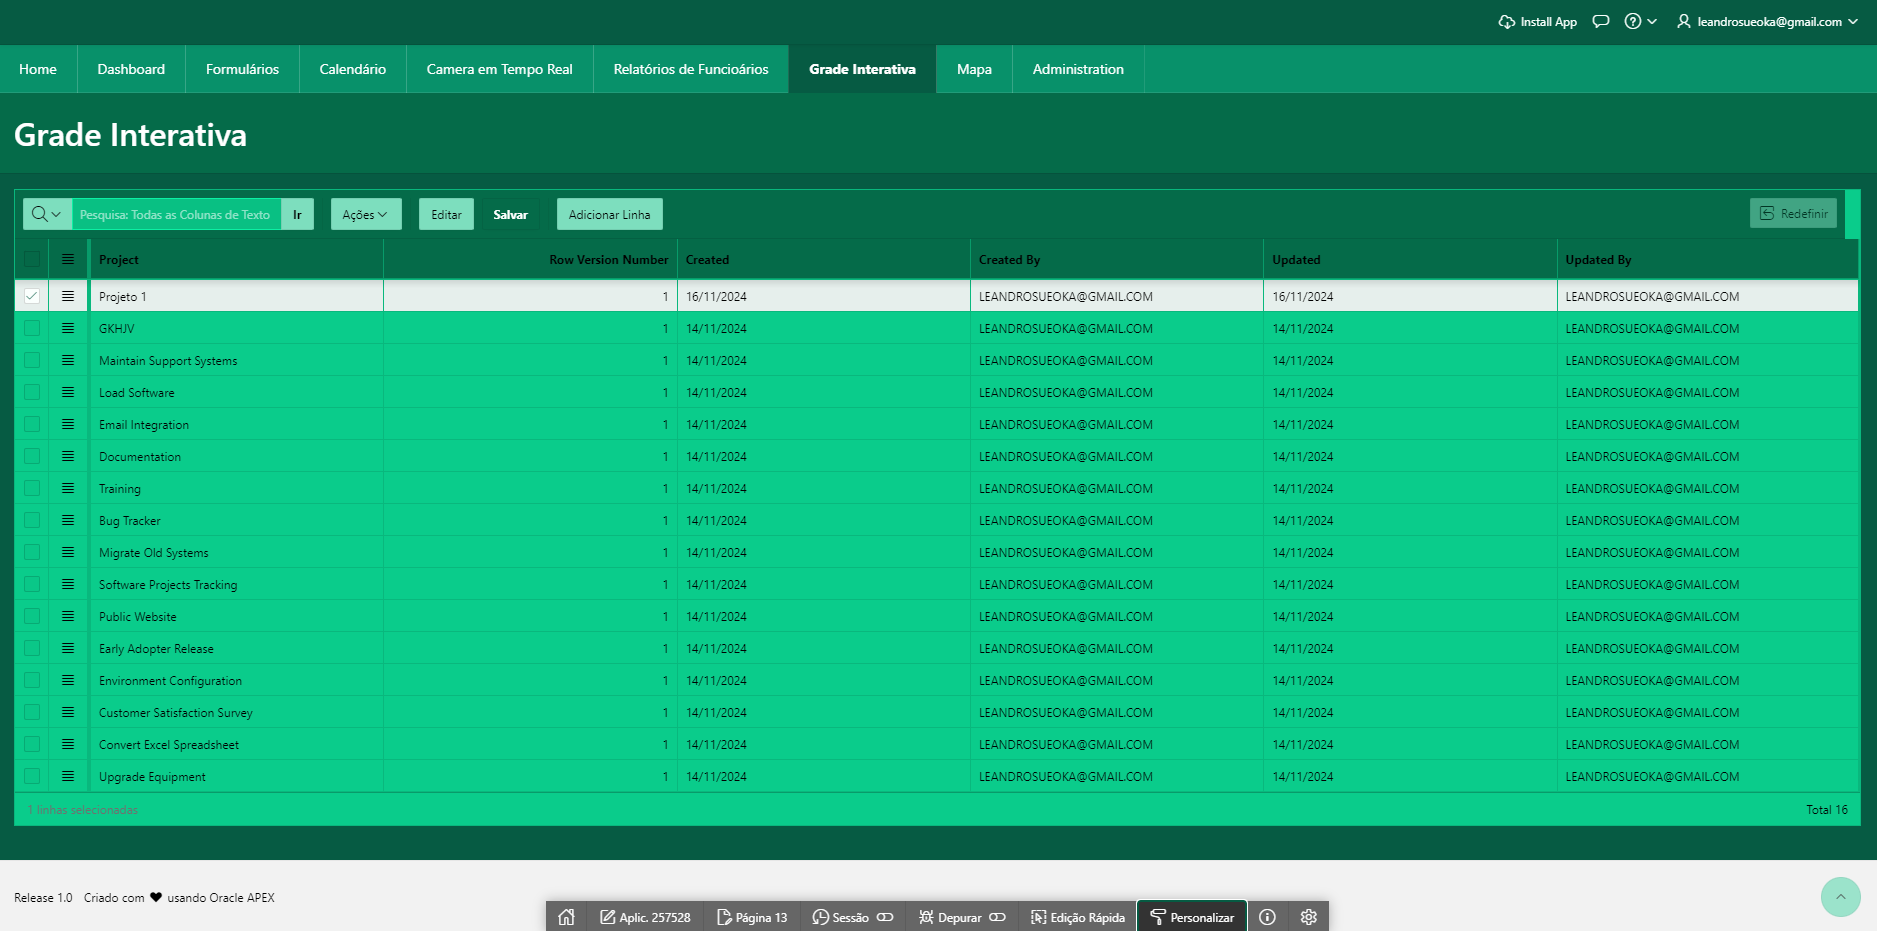
\includegraphics[scale=0.2]{Illustrations/Tela_grade_interativa.png}
\SourceOrNote{Autoria Própria (2024)}
\end{figure}
    
Temos uma tela de grade interativa que exibe diversas informações presentes no banco de dados. Estas informações podem ser filtradas diretamente na tela de forma simples e intuitiva.
\clearpage
\begin{figure}[!h]
\centering
\caption{Tela de mapa}
\label{fig:picture23}
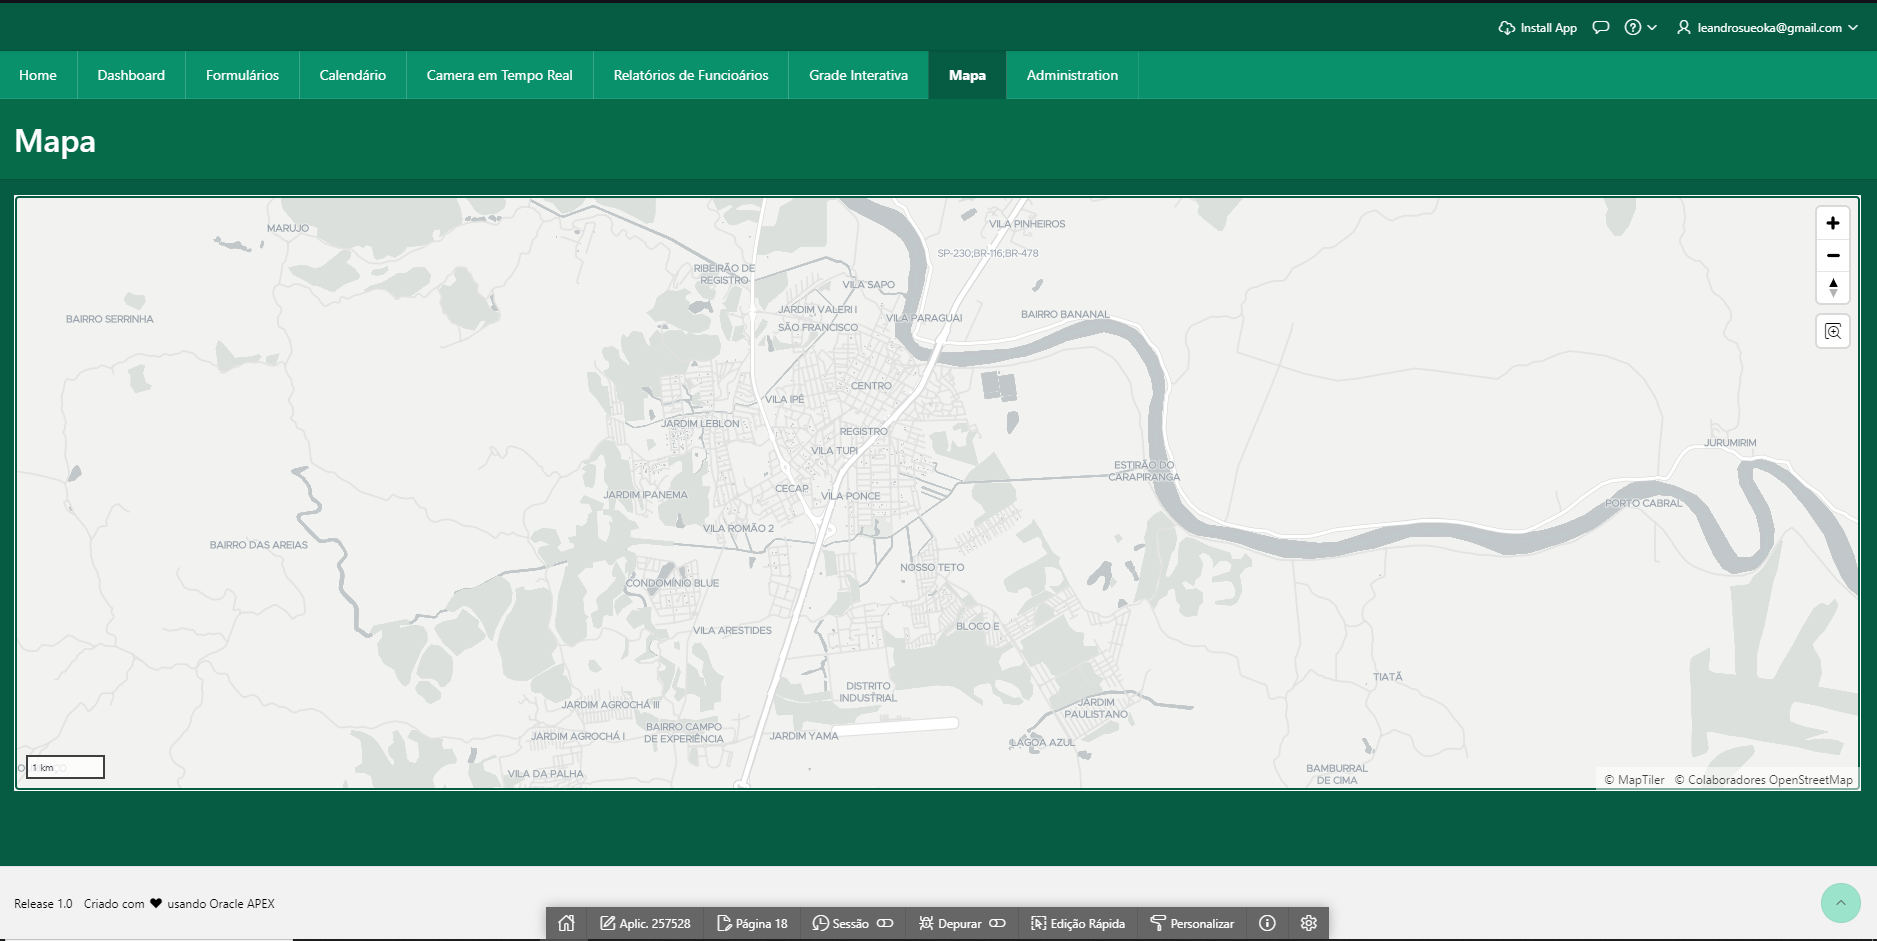
\includegraphics[scale=0.2]{Illustrations/Tela_mapa.png}
\SourceOrNote{Autoria Própria (2024)}
\end{figure}
        
O sistema conta também com uma tela de mapa, que exibe o local onde a(s) fazenda(s) vertical(is) estão situadas.

\begin{figure}[!h]
\centering
\caption{Tela de administração}
\label{fig:picture24}
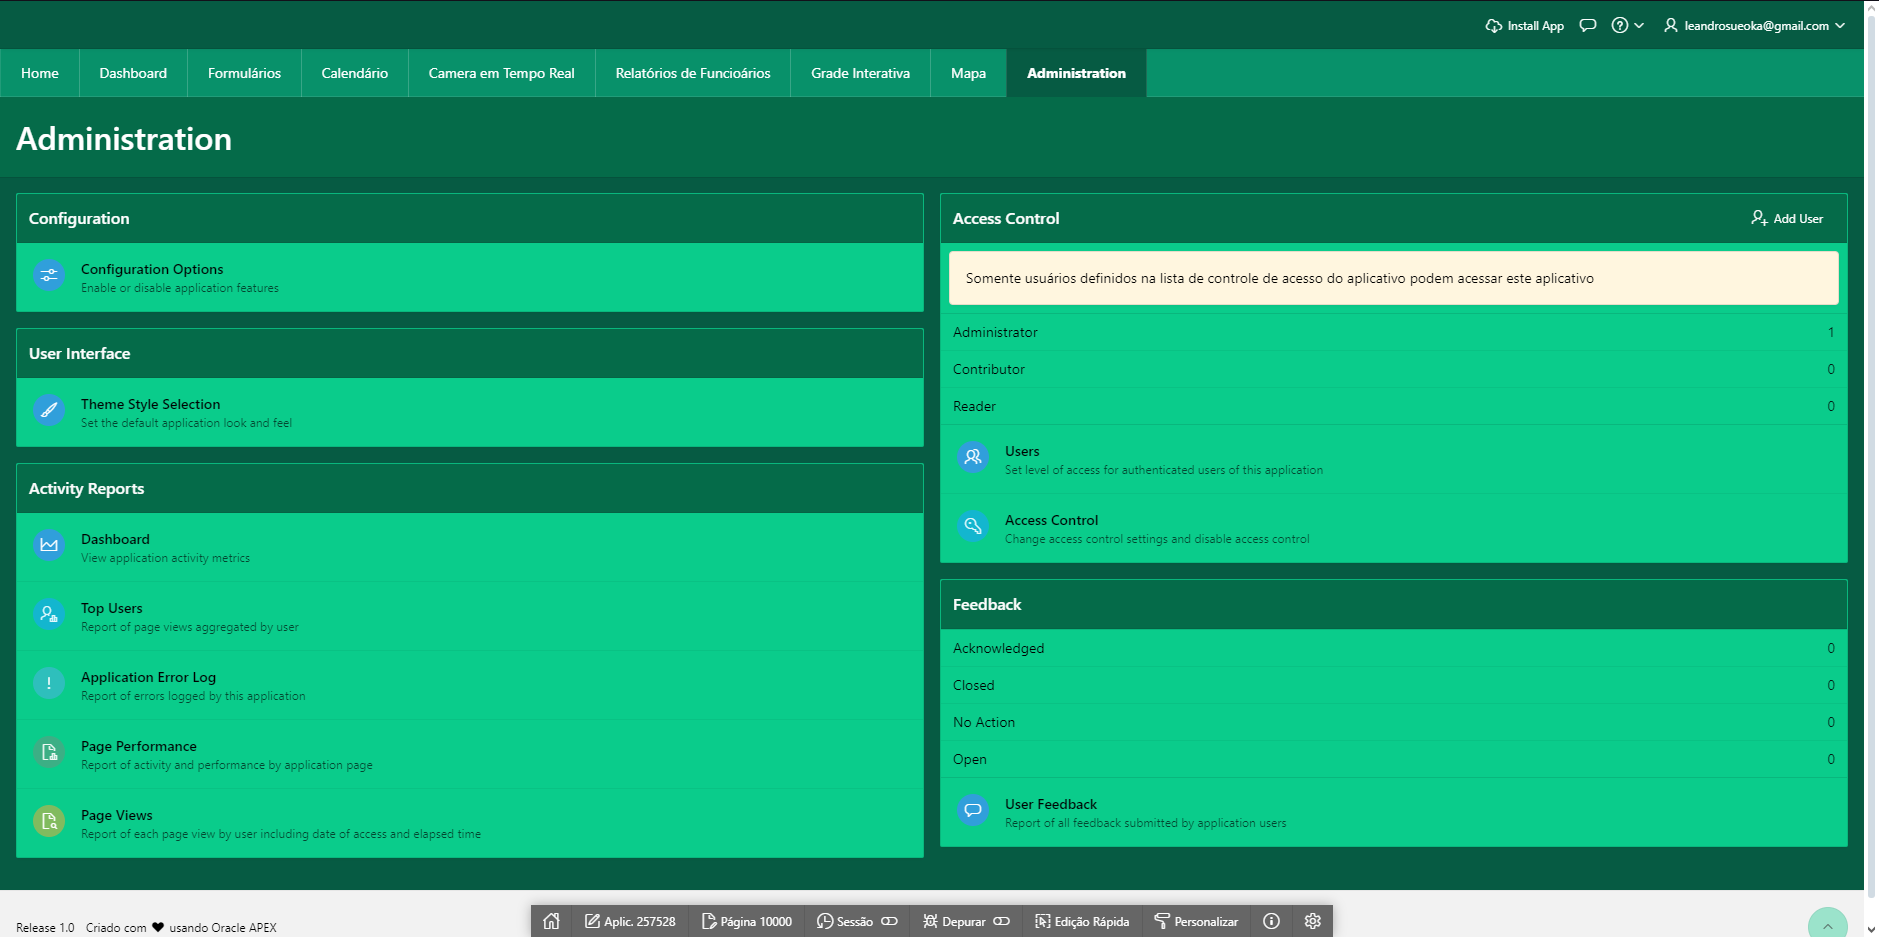
\includegraphics[scale=0.2]{Illustrations/Tela_adiministracao.png}
\SourceOrNote{Autoria Própria (2024)}
\end{figure}
            
O sistema conta com uma tela de administração onde o usuário pode personalizar algumas opções da aplicação (configuração e opções, seleção de tema, relatórios de atividades envolvendo dashboards, páginas visualizadas por usuário, log de erros, performance da página, visualizações, controle de acesso e opções de feedback referente o aplicativo).

\begin{figure}[!h]
\centering
\caption{Tela de calendario}
\label{fig:picture25}
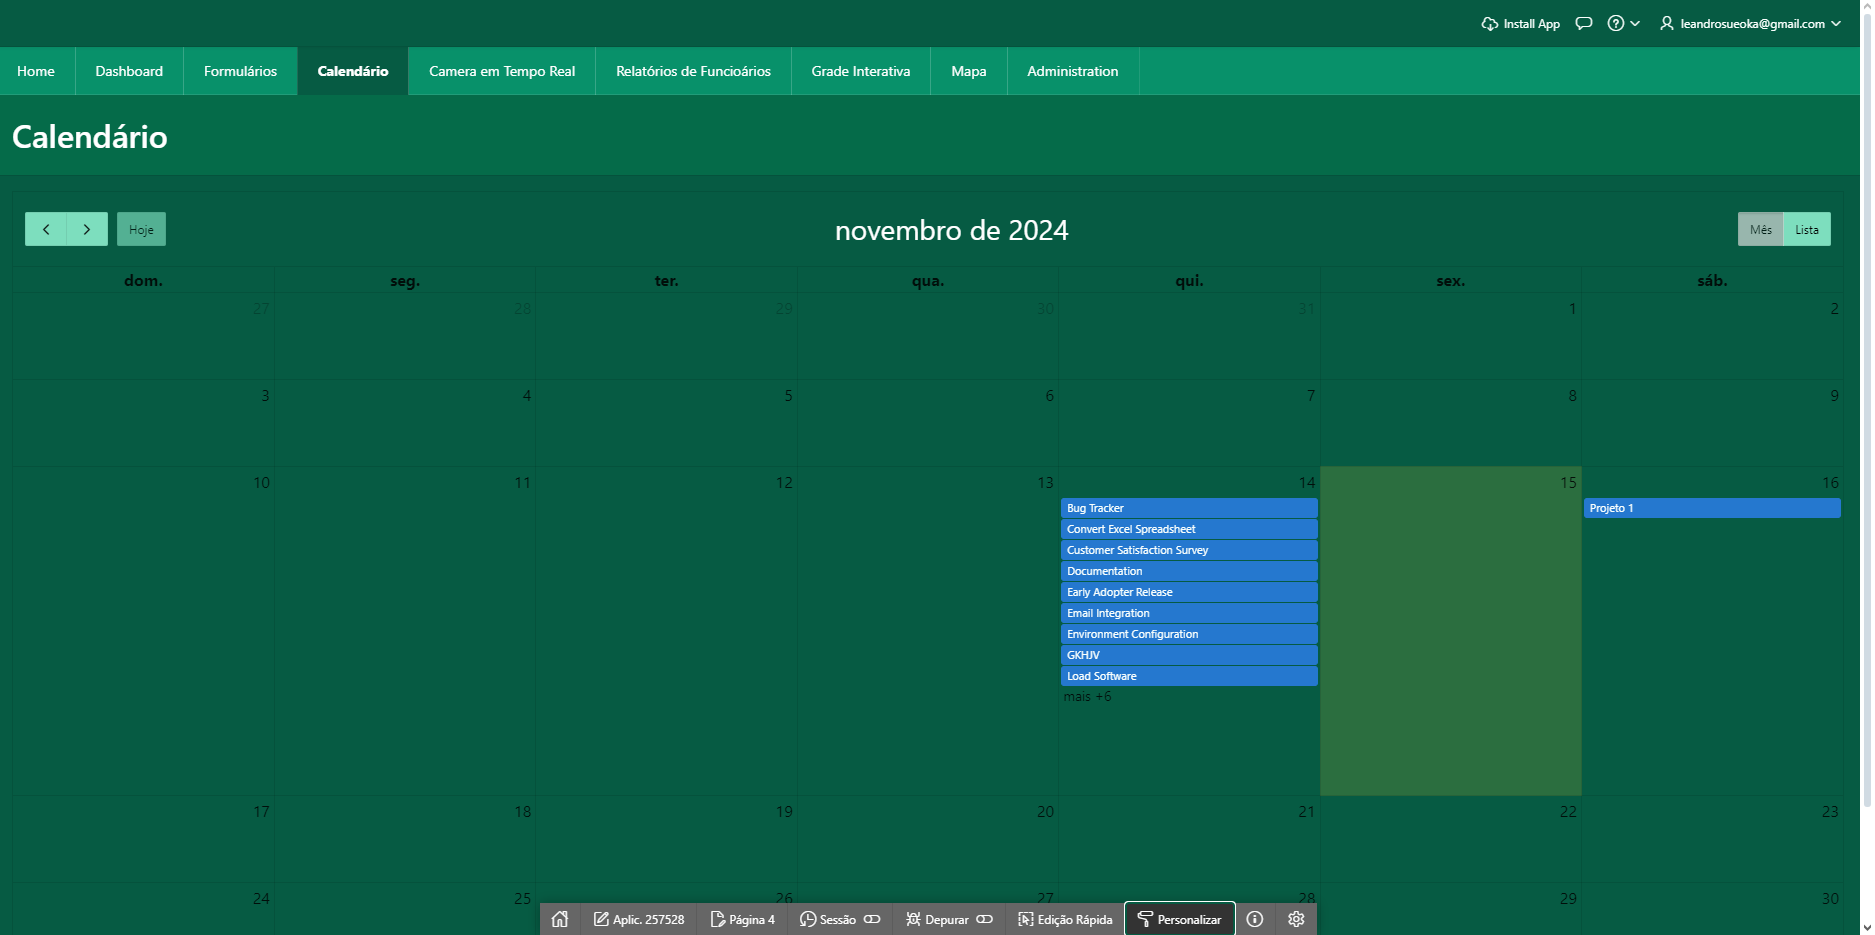
\includegraphics[scale=0.2]{Illustrations/Tela_calendario.png}
\SourceOrNote{Autoria Própria (2024)}
\end{figure}
                
O sistema também conta com uma tela de calendário, onde o usuário pode realizar quaisquer tipos de anotações referentes a fazenda vertical em função do tempo.

\subsection*{SITE}

Com o intuito de apresentar o projeto e a equipe envolvida foi desenvolvido um site.

\begin{figure}[!h]
\centering
\caption{Site}
\label{fig:picture26}
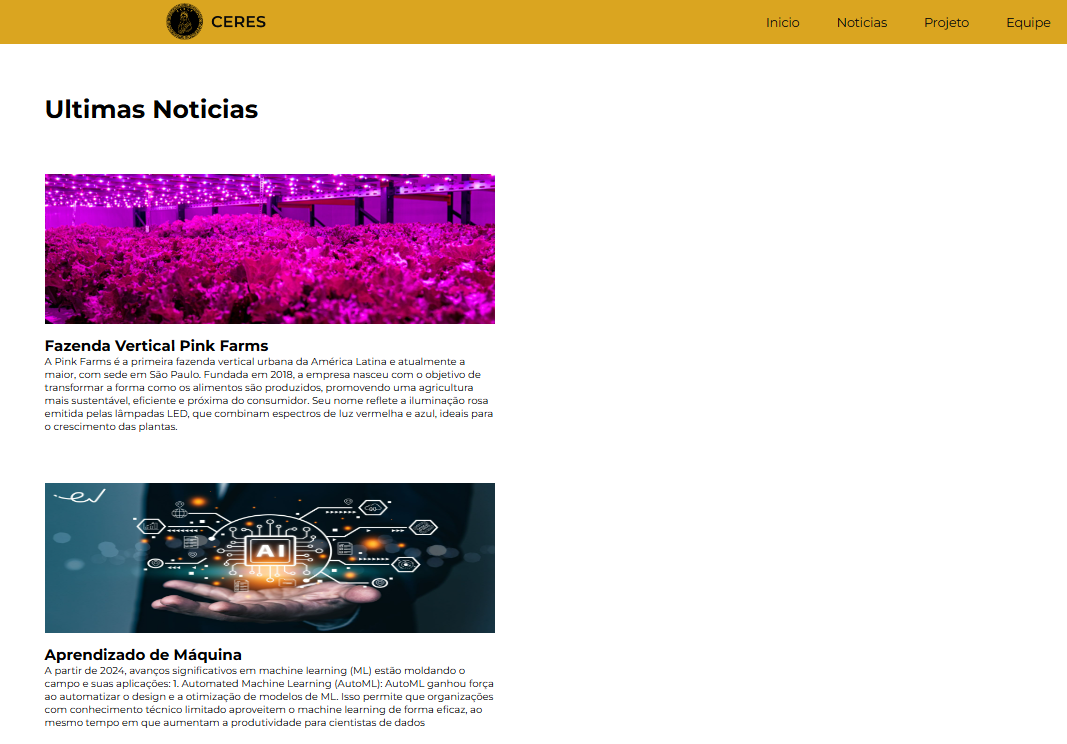
\includegraphics[scale=0.5]{Illustrations/site.png}
\SourceOrNote{Autoria Própria (2024)}
\end{figure}
O site tem uma página e foi desenvolvido em HTML. Na barra superior conta com um menu com quatro botões (Início, notícias, Projeto e equipe). Cada é um atalho para o trecho designado no site. 